\documentclass[lettersize,10pt]{article}

\usepackage{amsmath,amssymb}
\usepackage{graphicx}
\usepackage{booktabs}
\usepackage{longtable}
\usepackage{multirow}
\usepackage{xcolor}
\usepackage[caption=false,font=normalsize,labelfont=sf,textfont=sf]{subfig}
\usepackage{geometry}
\geometry{margin=1in}
\usepackage{hyperref}
\usepackage[protrusion=true,expansion=true]{microtype}

% Reduce blank pages from floats
\renewcommand{\topfraction}{0.9}
\renewcommand{\bottomfraction}{0.9}
\renewcommand{\textfraction}{0.1}
\renewcommand{\floatpagefraction}{0.7}

\title{Supplementary Material:\\An Explainable Evolutionary Grammar Approach\\for Interpretable Data Stream Classification with Concept Drift}
\author{Leandro Maciel Almeida and Leandro L. Minku}
\date{}

\begin{document}
\maketitle

\noindent This supplementary material provides extended experimental results, detailed statistical analyses, and per-dataset visualizations supporting the main paper. All sections are numbered with the prefix ``S'' to distinguish them from the main manuscript.

\tableofcontents
\clearpage


\section{Experimental Details}
\label{sec:s1}
\subsection{Dataset Dimensions}
\label{sec:s1_datasets}
The experimental evaluation encompasses 48 datasets: 41 binary classification and 7 multiclass datasets. Table~\ref{tab:s_drift_counts} shows the distribution across drift types.

\begin{table}[htbp]
\centering
\caption{Dataset Distribution by Drift Type}
\label{tab:s_drift_counts}
\begin{tabular}{lcc}
\toprule
\textbf{Drift Type} & \textbf{All} & \textbf{Binary Only} \\
\midrule
Abrupt & 16 & 14 \\
Gradual & 11 & 9 \\
Noisy & 8 & 8 \\
Stationary & 9 & 6 \\
Real & 4 & 4 \\
\midrule
Total & 48 & 41 \\
\bottomrule
\end{tabular}
\end{table}

The 7 multiclass datasets are: LED\_Abrupt\_Simple, LED\_Gradual\_Simple, LED\_Stationary, RBF\_Stationary, WAVEFORM\_Abrupt\_Simple, WAVEFORM\_Gradual\_Simple, and WAVEFORM\_Stationary. IntelLabSensors was excluded from all analyses due to data quality issues.

\subsection{Experimental Configurations}
\label{sec:s1_configs}
Table~\ref{tab:s_configs} summarizes the seven EGIS configurations evaluated. All configurations use a stream of 12{,}000 instances divided into chunks of the specified size.

\begin{table}[htbp]
\centering
\caption{EGIS Experimental Configurations}
\label{tab:s_configs}
\footnotesize
\begin{tabular}{lcccc}
\toprule
\textbf{Label} & \textbf{Chunk Size} & \textbf{Penalty ($\gamma$)} & \textbf{Num Chunks} & \textbf{Total Instances} \\
\midrule
EXP-1000-NP & 1000 & 0.0 & 12 & 12{,}000 \\
EXP-1000-P & 1000 & 0.1 & 12 & 12{,}000 \\
EXP-2000-NP & 2000 & 0.0 & 6 & 12{,}000 \\
EXP-2000-P & 2000 & 0.1 & 6 & 12{,}000 \\
EXP-500-NP & 500 & 0.0 & 24 & 12{,}000 \\
EXP-500-P & 500 & 0.1 & 24 & 12{,}000 \\
EXP-500-P03 & 500 & 0.3 & 24 & 12{,}000 \\
\bottomrule
\end{tabular}
\end{table}

\subsection{EGIS Hyperparameters}
\label{sec:s1_params}
Table~\ref{tab:s_params} lists all EGIS hyperparameters, organized by functional group. These settings were held constant across all seven configurations; only chunk size and complexity penalty ($\gamma$) vary.

\begin{table}[htbp]
\centering
\caption{EGIS Hyperparameter Settings}
\label{tab:s_params}
\footnotesize
\begin{tabular}{lc}
\toprule
\textbf{Parameter} & \textbf{Value} \\
\midrule
\multicolumn{2}{l}{\textit{Evolutionary Parameters}} \\
\midrule
Population size & 120 \\
Max generations & 200 \\
Max generations (recovery) & 25 \\
Elitism rate & 0.1 \\
Intelligent mutation rate & 0.8 \\
Tournament size (initial / final) & 2 / 5 \\
Balanced crossover & Yes \\
Max rules per class & 15 \\
Initial max depth & 10 \\
Stagnation threshold & 10 gen. \\
Early stopping patience & 20 gen. \\
Decision tree seeding ratio & 0.8 \\
DT seeding depths & 4, 7, 10, 13 \\
Adaptive seeding strategy & DT probe \\
\midrule
\multicolumn{2}{l}{\textit{Fitness Parameters}} \\
\midrule
Class coverage coefficient & 0.2 \\
G-Mean bonus coefficient & 0.1 \\
Regularization coefficient (initial) & 0.001 \\
Operator change coefficient & 0.05 \\
Complexity penalty ($\gamma$) & 0.0 / 0.1 / 0.3 \\
\midrule
\multicolumn{2}{l}{\textit{Drift Adaptation}} \\
\midrule
Drift severity classification & Custom \\
Severity levels & STABLE / MILD / MODERATE / SEVERE \\
Drift penalty reduction threshold & 0.1 \\
Recovery mutation override rate & 0.5 \\
Recovery random individual ratio & 0.6 \\
\midrule
\multicolumn{2}{l}{\textit{Memory Management}} \\
\midrule
Memory size (max) & 20 \\
Active pruning & Yes (age + fitness) \\
Max age & 10 chunks \\
Fitness threshold percentile & 0.25 \\
Abandon on severe drop & Yes ($<$0.55) \\
\bottomrule
\end{tabular}
\end{table}

Notably, EGIS does \textbf{not} rely on any external drift detection method. Instead, drift severity is classified by comparing the incoming data against known concept signatures stored in memory, yielding a four-level severity scale (STABLE, MILD, MODERATE, SEVERE) that governs the evolutionary response intensity.

\subsection{Baseline Model Configurations}
\label{sec:s1_baselines}
All baselines were evaluated under the same train-then-test protocol with pre-generated chunks. Table~\ref{tab:s_baselines_river} lists the River-based models and Table~\ref{tab:s_baselines_other} lists the remaining baselines.

\begin{table}[htbp]
\centering
\caption{River-Based Baseline Configurations}
\label{tab:s_baselines_river}
\footnotesize
\begin{tabular}{lccc}
\toprule
\textbf{Parameter} & \textbf{HAT} & \textbf{ARF} & \textbf{SRP} \\
\midrule
Framework & River 0.21+ & River 0.21+ & River 0.21+ \\
Constructor & \texttt{HoeffdingAdaptiveTreeClassifier()} & \texttt{ARFClassifier(n\_models=10)} & \texttt{SRPClassifier(n\_models=10)} \\
Ensemble size & 1 (single tree) & 10 & 10 \\
All other params & River defaults & River defaults & River defaults \\
Drift handling & Built-in & Built-in & Built-in \\
\bottomrule
\end{tabular}
\end{table}

\begin{table}[htbp]
\centering
\caption{Other Baseline Configurations}
\label{tab:s_baselines_other}
\footnotesize
\begin{tabular}{lcccc}
\toprule
\textbf{Parameter} & \textbf{ROSE} & \textbf{ACDWM} & \textbf{ERulesD2S} & \textbf{CDCMS} \\
\midrule
Framework & MOA (Java) & Python (DWMIL) & MOA + JCLEC4 & MOA fork \\
Execution & MOA CLI subprocess & \texttt{baseline\_acdwm.py} & \texttt{erulesd2s\_wrapper.py} & \texttt{Setup\_CDCMS\_CIL.ipynb} \\
Key params & MOA defaults & $\theta$=0.001, err=gm, r=1.0 & -s\,25 -g\,50 -r\,5 & CDCMS\_CIL\_GMean \\
Scope & All datasets & Binary only (41) & All datasets & All datasets \\
\bottomrule
\end{tabular}
\end{table}

\textbf{HAT} (Hoeffding Adaptive Tree) is a single incremental decision tree instantiated with all River default parameters, including built-in drift handling. \textbf{ARF} (Adaptive Random Forest) and \textbf{SRP} (Streaming Random Patches) are ensemble methods with 10 base learners (\texttt{n\_models=10}); all other parameters use River defaults, including built-in drift handling. \textbf{ROSE} (Robust Online Self-Adjusting Ensemble) is executed as a Java subprocess via the MOA command line with default parameters and \texttt{WindowAUCImbalancedPerformanceEvaluator} for binary datasets (Cano and Krawczyk, 2022). \textbf{ACDWM} (Adaptive Concept Drift-aware Weighted Majority) employs Dynamic Weighted Majority with UnderBagging via the DWMIL library; it supports binary classification only (41 datasets). \textbf{ERulesD2S} is an evolutionary rule learner via MOA/JCLEC4 with population size 25, 50 generations, and 5 rules per class. \textbf{CDCMS} (Concept-Drift Class-specific Module Switching) is a MOA-based approach using the G-Mean variant (CDCMS\_CIL\_GMean) with a custom evaluator.

\subsection{Computational Environment}
\label{sec:s1_environment}
All experiments were executed on Google Colab instances with a T4 GPU and approximately 12\,GB of RAM. Python~3.10+ with River~0.23+ was used for EGIS, HAT, ARF, SRP, ROSE, and ACDWM. Java-based models (ERulesD2S, CDCMS) ran on OpenJDK within the same Colab environment.

Per-dataset timeout limits were enforced to ensure tractable execution: ROSE, ARF, SRP, and ACDWM had a 600\,s limit; HAT had 300\,s; ERulesD2S had 1800\,s due to its slower Java-based evolutionary process. All models were evaluated using the same train-then-test protocol with pre-generated chunks, ensuring identical training and testing data across methods. The primary evaluation metric is G-Mean, with Accuracy and weighted F1 reported as secondary metrics.


\section{Complete Performance Tables}
\label{sec:s2}
This section provides the complete per-dataset G-Mean performance tables for all three no-penalty configurations, covering all 41 binary datasets and all 8 models. Each table includes per-row bolding of the best result, win/loss/draw counts for EGIS versus each baseline, and average Friedman rankings. These tables extend the summary statistics presented in the main paper.

\subsection{Per-Dataset G-Mean: Chunk Size 500 (EXP-500-NP)}
\label{sec:s2_exp_500_np}

\scriptsize
\begin{longtable}{lcccccccc}
\caption{Per-Dataset G-Mean: Binary Datasets (EXP-500-NP)}\label{tab:s_binary_exp_500_np} \\
\toprule
\textbf{Dataset} & \textbf{EGIS} & \textbf{ARF} & \textbf{SRP} & \textbf{HAT} & \textbf{ROSE} & \textbf{ACDWM} & \textbf{ERulesD2S} & \textbf{CDCMS} \\
\midrule
\endfirsthead
\toprule
\textbf{Dataset} & \textbf{EGIS} & \textbf{ARF} & \textbf{SRP} & \textbf{HAT} & \textbf{ROSE} & \textbf{ACDWM} & \textbf{ERulesD2S} & \textbf{CDCMS} \\
\midrule
\endhead
\midrule \multicolumn{9}{l}{\textit{Abrupt Drift (14)}}\\
\midrule
AGR\_Ab\_Chain\_L & \textbf{0.8881} & 0.7878 & 0.7846 & 0.6645 & 0.8301 & 0.8558 & 0.5285 & 0.6552 \\
AGR\_Ab\_Mild & \textbf{0.9055} & 0.8249 & 0.8662 & 0.5850 & 0.9005 & 0.8882 & 0.5420 & 0.6280 \\
AGR\_Ab\_Severe & 0.8997 & 0.8398 & 0.8894 & 0.6800 & \textbf{0.9250} & 0.8905 & 0.5432 & 0.6941 \\
HYP\_Ab\_Simple & 0.7555 & 0.8354 & 0.7713 & 0.8822 & 0.8634 & 0.7970 & 0.5252 & \textbf{0.9039} \\
RT\_Ab\_Recur. & 0.6149 & 0.5333 & 0.5242 & 0.5334 & 0.6540 & \textbf{0.6851} & 0.5519 & 0.5386 \\
RT\_Ab\_Simple & 0.6139 & 0.5499 & 0.5113 & 0.5423 & 0.6595 & \textbf{0.6840} & 0.5416 & 0.5281 \\
RBF\_Ab\_Blip & 0.8318 & 0.9102 & \textbf{0.9162} & 0.8371 & 0.8960 & 0.8700 & 0.5212 & 0.8540 \\
RBF\_Ab\_Severe & 0.8069 & 0.8938 & \textbf{0.9015} & 0.7893 & 0.8697 & 0.8417 & 0.5217 & 0.7948 \\
SEA\_Ab\_Chain & 0.9472 & 0.9718 & 0.9557 & 0.9303 & \textbf{0.9774} & 0.9263 & 0.6232 & 0.9361 \\
SEA\_Ab\_Recur. & 0.9452 & \textbf{0.9772} & 0.9392 & 0.9459 & 0.9755 & 0.9313 & 0.6460 & 0.9540 \\
SEA\_Ab\_Simple & 0.9496 & 0.9772 & 0.9731 & 0.9524 & \textbf{0.9785} & 0.9362 & 0.6204 & 0.9412 \\
SINE\_Ab\_Simple & 0.9510 & \textbf{0.9881} & 0.9868 & 0.9708 & 0.9796 & 0.9427 & 0.6547 & 0.9766 \\
STAG\_Ab\_Chain & 0.9676 & \textbf{0.9943} & 0.9929 & 0.7630 & 0.9215 & 0.8952 & 0.7776 & 0.9825 \\
STAG\_Ab\_Recur. & 0.9565 & 0.9969 & 0.9889 & 0.7902 & \textbf{0.9973} & 0.9167 & 0.7969 & 0.9895 \\
\midrule \multicolumn{9}{l}{\textit{Gradual Drift (9)}}\\
\midrule
HYP\_Gr\_Simple & 0.7555 & 0.8316 & 0.7744 & 0.8792 & 0.8634 & 0.7986 & 0.5361 & \textbf{0.9039} \\
RT\_Gr\_Simple & 0.6099 & 0.5485 & 0.5113 & 0.5229 & 0.6688 & \textbf{0.6974} & 0.5612 & 0.5257 \\
RBF\_Gr\_Mod. & 0.8191 & 0.8945 & \textbf{0.9044} & 0.8197 & 0.8893 & 0.8501 & 0.5347 & 0.8234 \\
RBF\_Gr\_Severe & 0.8232 & \textbf{0.9025} & 0.8966 & 0.8298 & 0.8944 & 0.8513 & 0.5259 & 0.8196 \\
SEA\_Gr\_Recur. & 0.9388 & \textbf{0.9613} & 0.9539 & 0.9202 & 0.9596 & 0.9156 & 0.6350 & 0.9221 \\
SEA\_Gr\_Fast & 0.9529 & 0.9771 & 0.9765 & 0.9501 & \textbf{0.9795} & 0.9385 & 0.6384 & 0.9558 \\
SEA\_Gr\_Slow & 0.9566 & 0.9775 & 0.9761 & 0.9477 & \textbf{0.9811} & 0.9385 & 0.6326 & 0.9358 \\
SINE\_Gr\_Recur. & 0.9173 & \textbf{0.9522} & 0.9501 & 0.9285 & 0.9428 & 0.9001 & 0.6359 & 0.9237 \\
STAG\_Gr\_Chain & 0.9195 & \textbf{0.9500} & 0.9360 & 0.6859 & 0.9203 & 0.8385 & 0.7637 & 0.9188 \\
\midrule \multicolumn{9}{l}{\textit{Noisy Drift (8)}}\\
\midrule
AGR\_Ab\_Sev\_N & 0.9173 & 0.7790 & 0.8356 & 0.6868 & \textbf{0.9401} & 0.8867 & 0.5474 & 0.6622 \\
HYP\_Gr\_Noise & 0.7527 & 0.8115 & 0.7591 & 0.8556 & 0.8478 & 0.7837 & 0.5295 & \textbf{0.8734} \\
RT\_Gr\_Noise & 0.6202 & 0.5112 & 0.4766 & 0.5322 & 0.6902 & \textbf{0.6903} & 0.5502 & 0.5196 \\
RBF\_Ab\_Blip\_N & 0.8267 & 0.9040 & \textbf{0.9046} & 0.8254 & 0.8859 & 0.8592 & 0.5228 & 0.8500 \\
RBF\_Gr\_Sev\_N & 0.8242 & 0.8903 & \textbf{0.9012} & 0.8177 & 0.8771 & 0.8527 & 0.5184 & 0.8226 \\
SEA\_Ab\_Ch\_N & 0.9458 & 0.9655 & 0.9374 & 0.9172 & \textbf{0.9712} & 0.9215 & 0.6324 & 0.9281 \\
SINE\_Ab\_Rec\_N & 0.9133 & 0.9807 & \textbf{0.9813} & 0.9491 & 0.9731 & 0.8994 & 0.6678 & 0.9464 \\
STAG\_Ab\_Ch\_N & 0.9647 & \textbf{0.9953} & 0.9817 & 0.7584 & 0.9216 & 0.8981 & 0.7737 & 0.9428 \\
\midrule \multicolumn{9}{l}{\textit{Stationary Drift (6)}}\\
\midrule
AGR\_Station. & \textbf{1.0000} & 0.9335 & 0.9983 & 0.9813 & 0.9967 & 0.9583 & 0.5239 & 0.9868 \\
HYP\_Station. & 0.7229 & 0.8185 & 0.7621 & 0.8745 & 0.8523 & 0.7818 & 0.5259 & \textbf{0.9044} \\
RT\_Station. & 0.5425 & 0.5852 & 0.5550 & 0.4321 & \textbf{0.5941} & 0.5748 & 0.5278 & 0.5157 \\
SEA\_Station. & 0.9544 & 0.9798 & 0.9620 & 0.9505 & \textbf{0.9836} & 0.9433 & 0.6123 & 0.9460 \\
SINE\_Station. & 0.9531 & 0.9858 & \textbf{0.9867} & 0.9684 & 0.9824 & 0.9436 & 0.6348 & 0.9798 \\
STAG\_Station. & \textbf{1.0000} & 0.9980 & 0.9975 & 0.8009 & 0.9994 & 0.9583 & 0.7872 & \textbf{1.0000} \\
\midrule \multicolumn{9}{l}{\textit{Real-World Drift (4)}}\\
\midrule
AssetNeg\_F2 & 0.9494 & 0.9672 & 0.9717 & 0.9472 & \textbf{0.9820} & 0.9425 & 0.6512 & 0.9495 \\
AssetNeg\_F3 & \textbf{0.9952} & 0.9656 & 0.9215 & 0.9614 & 0.9922 & 0.9577 & 0.7623 & 0.9468 \\
AssetNeg\_F4 & 0.9055 & 0.9464 & 0.9362 & 0.9395 & 0.6618 & 0.9134 & 0.5616 & \textbf{0.9502} \\
Electricity & 0.7096 & 0.8865 & 0.8851 & 0.8614 & \textbf{0.9053} & 0.7162 & 0.6193 & 0.8570 \\
\midrule
\textbf{EGIS W/L/D} & -- & 11/30/0 & 13/28/0 & 26/15/0 & 8/33/0 & 24/17/0 & 41/0/0 & 22/18/1 \\
\textbf{Mean} & 0.8591 & 0.8776 & 0.8691 & 0.8149 & 0.8923 & 0.8603 & 0.6050 & 0.8460 \\
\textbf{Std} & 0.1247 & 0.1405 & 0.1498 & 0.1502 & 0.1109 & 0.0929 & 0.0866 & 0.1518 \\
\textbf{Avg Rank} & 4.45 & 2.85 & 3.68 & 5.49 & 2.41 & 4.95 & 7.51 & 4.65 \\
\bottomrule
\end{longtable}
\normalsize

\subsection{Per-Dataset G-Mean: Chunk Size 1000 (EXP-1000-NP)}
\label{sec:s2_exp_1000_np}

\scriptsize
\begin{longtable}{lcccccccc}
\caption{Per-Dataset G-Mean: Binary Datasets (EXP-1000-NP)}\label{tab:s_binary_exp_1000_np} \\
\toprule
\textbf{Dataset} & \textbf{EGIS} & \textbf{ARF} & \textbf{SRP} & \textbf{HAT} & \textbf{ROSE} & \textbf{ACDWM} & \textbf{ERulesD2S} & \textbf{CDCMS} \\
\midrule
\endfirsthead
\toprule
\textbf{Dataset} & \textbf{EGIS} & \textbf{ARF} & \textbf{SRP} & \textbf{HAT} & \textbf{ROSE} & \textbf{ACDWM} & \textbf{ERulesD2S} & \textbf{CDCMS} \\
\midrule
\endhead
\midrule \multicolumn{9}{l}{\textit{Abrupt Drift (14)}}\\
\midrule
AGR\_Ab\_Chain\_L & \textbf{0.8723} & 0.7897 & 0.8606 & 0.6756 & 0.8301 & 0.7417 & 0.5260 & 0.6234 \\
AGR\_Ab\_Mild & \textbf{0.9117} & 0.7989 & 0.8028 & 0.6456 & 0.9005 & 0.8278 & 0.5373 & 0.6127 \\
AGR\_Ab\_Severe & 0.9020 & 0.8471 & 0.8566 & 0.6902 & \textbf{0.9250} & 0.8341 & 0.5374 & 0.6908 \\
HYP\_Ab\_Simple & 0.7812 & 0.8306 & 0.7728 & 0.8771 & 0.8634 & 0.7670 & 0.5242 & \textbf{0.8993} \\
RT\_Ab\_Recur. & 0.6448 & 0.5611 & 0.5298 & 0.5198 & 0.6540 & \textbf{0.6695} & 0.5479 & 0.5168 \\
RT\_Ab\_Simple & 0.6489 & 0.5479 & 0.5012 & 0.4922 & 0.6595 & \textbf{0.6697} & 0.5497 & 0.5330 \\
RBF\_Ab\_Blip & 0.8578 & 0.9140 & \textbf{0.9154} & 0.8360 & 0.8960 & 0.8300 & 0.5273 & 0.8413 \\
RBF\_Ab\_Severe & 0.8322 & \textbf{0.8978} & 0.8958 & 0.8117 & 0.8697 & 0.7758 & 0.5080 & 0.7810 \\
SEA\_Ab\_Chain & 0.9616 & 0.9721 & 0.9308 & 0.9295 & \textbf{0.9774} & 0.8787 & 0.6181 & 0.9343 \\
SEA\_Ab\_Recur. & 0.9659 & \textbf{0.9765} & 0.9309 & 0.9452 & 0.9755 & 0.8900 & 0.6441 & 0.9582 \\
SEA\_Ab\_Simple & 0.9635 & 0.9752 & 0.9608 & 0.9487 & \textbf{0.9785} & 0.8962 & 0.6166 & 0.9415 \\
SINE\_Ab\_Simple & 0.9639 & \textbf{0.9873} & 0.9864 & 0.9747 & 0.9796 & 0.9016 & 0.6497 & 0.9747 \\
STAG\_Ab\_Chain & 0.9311 & \textbf{0.9951} & 0.9925 & 0.7811 & 0.9215 & 0.7899 & 0.7563 & 0.9680 \\
STAG\_Ab\_Recur. & 0.9091 & \textbf{0.9975} & 0.9905 & 0.7858 & 0.9973 & 0.8333 & 0.7630 & 0.9780 \\
\midrule \multicolumn{9}{l}{\textit{Gradual Drift (9)}}\\
\midrule
HYP\_Gr\_Simple & 0.7810 & 0.8369 & 0.7712 & 0.8787 & 0.8634 & 0.7719 & 0.5399 & \textbf{0.8993} \\
RT\_Gr\_Simple & 0.6539 & 0.5131 & 0.4874 & 0.5271 & 0.6688 & \textbf{0.7005} & 0.5368 & 0.5523 \\
RBF\_Gr\_Mod. & 0.8474 & 0.8961 & \textbf{0.9024} & 0.8193 & 0.8893 & 0.8126 & 0.5144 & 0.8307 \\
RBF\_Gr\_Severe & 0.8476 & 0.9051 & \textbf{0.9051} & 0.8251 & 0.8944 & 0.8172 & 0.5203 & 0.8470 \\
SEA\_Gr\_Recur. & 0.9424 & 0.9594 & 0.9334 & 0.9143 & \textbf{0.9596} & 0.8754 & 0.6480 & 0.9073 \\
SEA\_Gr\_Fast & 0.9654 & 0.9777 & 0.9323 & 0.9470 & \textbf{0.9795} & 0.8991 & 0.6004 & 0.9513 \\
SEA\_Gr\_Slow & 0.9625 & 0.9774 & 0.9716 & 0.9446 & \textbf{0.9811} & 0.9011 & 0.6285 & 0.9366 \\
SINE\_Gr\_Recur. & 0.9227 & \textbf{0.9519} & 0.9504 & 0.9356 & 0.9428 & 0.8620 & 0.6455 & 0.9168 \\
STAG\_Gr\_Chain & 0.8783 & \textbf{0.9486} & 0.9428 & 0.7221 & 0.9203 & 0.7276 & 0.7805 & 0.9043 \\
\midrule \multicolumn{9}{l}{\textit{Noisy Drift (8)}}\\
\midrule
AGR\_Ab\_Sev\_N & 0.9281 & 0.8094 & 0.7486 & 0.6597 & \textbf{0.9401} & 0.8355 & 0.5454 & 0.6366 \\
HYP\_Gr\_Noise & 0.7582 & 0.8224 & 0.7634 & 0.8550 & 0.8478 & 0.7560 & 0.5371 & \textbf{0.8757} \\
RT\_Gr\_Noise & 0.6509 & 0.5315 & 0.4635 & 0.5518 & 0.6902 & \textbf{0.7049} & 0.5359 & 0.5456 \\
RBF\_Ab\_Blip\_N & 0.8530 & 0.9021 & \textbf{0.9042} & 0.8238 & 0.8859 & 0.8310 & 0.5192 & 0.8337 \\
RBF\_Gr\_Sev\_N & 0.8421 & 0.8961 & \textbf{0.8999} & 0.8157 & 0.8771 & 0.8180 & 0.5256 & 0.8192 \\
SEA\_Ab\_Ch\_N & 0.9568 & 0.9681 & 0.9360 & 0.9287 & \textbf{0.9712} & 0.8762 & 0.5975 & 0.9252 \\
SINE\_Ab\_Rec\_N & 0.8840 & 0.9799 & \textbf{0.9811} & 0.9533 & 0.9731 & 0.8184 & 0.6275 & 0.9255 \\
STAG\_Ab\_Ch\_N & 0.9325 & \textbf{0.9951} & 0.9868 & 0.7640 & 0.9216 & 0.7902 & 0.7769 & 0.9211 \\
\midrule \multicolumn{9}{l}{\textit{Stationary Drift (6)}}\\
\midrule
AGR\_Station. & \textbf{1.0000} & 0.9409 & 0.9984 & 0.9796 & 0.9967 & 0.9167 & 0.5308 & 0.9958 \\
HYP\_Station. & 0.7371 & 0.8199 & 0.7624 & 0.8806 & 0.8523 & 0.7452 & 0.5248 & \textbf{0.9104} \\
RT\_Station. & 0.5606 & 0.5838 & 0.5398 & 0.4957 & 0.5941 & \textbf{0.6398} & 0.5141 & 0.5020 \\
SEA\_Station. & 0.9714 & 0.9795 & 0.9499 & 0.9581 & \textbf{0.9836} & 0.9034 & 0.6251 & 0.9519 \\
SINE\_Station. & 0.9665 & 0.9868 & \textbf{0.9883} & 0.9711 & 0.9824 & 0.9040 & 0.6350 & 0.9799 \\
STAG\_Station. & \textbf{1.0000} & 0.9974 & 0.9970 & 0.8053 & 0.9994 & 0.9167 & 0.7609 & \textbf{1.0000} \\
\midrule \multicolumn{9}{l}{\textit{Real-World Drift (4)}}\\
\midrule
AssetNeg\_F2 & 0.9635 & 0.9583 & 0.9726 & 0.9514 & \textbf{0.9820} & 0.9050 & 0.6272 & 0.9397 \\
AssetNeg\_F3 & \textbf{0.9976} & 0.9573 & 0.9292 & 0.9673 & 0.9922 & 0.9161 & 0.7605 & 0.9589 \\
AssetNeg\_F4 & 0.9149 & 0.9469 & 0.9358 & 0.9394 & 0.6618 & 0.8776 & 0.5724 & \textbf{0.9500} \\
Electricity & 0.7739 & 0.8913 & 0.8543 & 0.8565 & \textbf{0.9053} & 0.7185 & 0.6385 & 0.8258 \\
\midrule
\textbf{EGIS W/L/D} & -- & 12/29/0 & 21/20/0 & 31/10/0 & 8/33/0 & 35/6/0 & 41/0/0 & 28/12/1 \\
\textbf{Mean} & 0.8692 & 0.8786 & 0.8618 & 0.8191 & 0.8923 & 0.8182 & 0.5994 & 0.8414 \\
\textbf{Std} & 0.1133 & 0.1395 & 0.1524 & 0.1462 & 0.1109 & 0.0781 & 0.0841 & 0.1520 \\
\textbf{Avg Rank} & 3.70 & 2.88 & 3.76 & 5.29 & 2.41 & 5.76 & 7.59 & 4.62 \\
\bottomrule
\end{longtable}
\normalsize

\subsection{Per-Dataset G-Mean: Chunk Size 2000 (EXP-2000-NP)}
\label{sec:s2_exp_2000_np}

\scriptsize
\begin{longtable}{lcccccccc}
\caption{Per-Dataset G-Mean: Binary Datasets (EXP-2000-NP)}\label{tab:s_binary_exp_2000_np} \\
\toprule
\textbf{Dataset} & \textbf{EGIS} & \textbf{ARF} & \textbf{SRP} & \textbf{HAT} & \textbf{ROSE} & \textbf{ACDWM} & \textbf{ERulesD2S} & \textbf{CDCMS} \\
\midrule
\endfirsthead
\toprule
\textbf{Dataset} & \textbf{EGIS} & \textbf{ARF} & \textbf{SRP} & \textbf{HAT} & \textbf{ROSE} & \textbf{ACDWM} & \textbf{ERulesD2S} & \textbf{CDCMS} \\
\midrule
\endhead
\midrule \multicolumn{9}{l}{\textit{Abrupt Drift (14)}}\\
\midrule
AGR\_Ab\_Chain\_L & 0.7610 & 0.7453 & 0.7460 & 0.6784 & \textbf{0.8301} & 0.6475 & 0.5248 & 0.5961 \\
AGR\_Ab\_Mild & 0.8331 & 0.8350 & 0.7006 & 0.6532 & \textbf{0.9005} & 0.7467 & 0.5366 & 0.5950 \\
AGR\_Ab\_Severe & 0.8524 & 0.8254 & 0.9187 & 0.6985 & \textbf{0.9250} & 0.7475 & 0.5433 & 0.6797 \\
HYP\_Ab\_Simple & 0.7889 & 0.8343 & 0.7733 & 0.8779 & 0.8634 & 0.6900 & 0.5335 & \textbf{0.9128} \\
RT\_Ab\_Recur. & \textbf{0.6739} & 0.5405 & 0.5146 & 0.5474 & 0.6540 & 0.6016 & 0.5424 & 0.5032 \\
RT\_Ab\_Simple & \textbf{0.6613} & 0.5520 & 0.5292 & 0.5509 & 0.6595 & 0.6446 & 0.5474 & 0.5301 \\
RBF\_Ab\_Blip & 0.8642 & 0.9035 & \textbf{0.9169} & 0.8370 & 0.8960 & 0.7516 & 0.5126 & 0.8461 \\
RBF\_Ab\_Severe & 0.7836 & \textbf{0.8936} & 0.8929 & 0.8130 & 0.8697 & 0.6835 & 0.5120 & 0.7986 \\
SEA\_Ab\_Chain & 0.9589 & 0.9758 & 0.9638 & 0.9263 & \textbf{0.9774} & 0.7861 & 0.6346 & 0.9240 \\
SEA\_Ab\_Recur. & 0.9652 & \textbf{0.9760} & 0.9000 & 0.9441 & 0.9755 & 0.8084 & 0.6237 & 0.9409 \\
SEA\_Ab\_Simple & 0.9587 & 0.9773 & 0.9782 & 0.9478 & \textbf{0.9785} & 0.8142 & 0.6313 & 0.9455 \\
SINE\_Ab\_Simple & 0.9749 & 0.9858 & \textbf{0.9872} & 0.9732 & 0.9796 & 0.8222 & 0.6422 & 0.9837 \\
STAG\_Ab\_Chain & 0.8479 & \textbf{0.9957} & 0.9920 & 0.7905 & 0.9215 & 0.7066 & 0.7553 & 0.9438 \\
STAG\_Ab\_Recur. & 0.8000 & 0.9970 & 0.9900 & 0.8014 & \textbf{0.9973} & 0.6667 & 0.7674 & 0.9516 \\
\midrule \multicolumn{9}{l}{\textit{Gradual Drift (9)}}\\
\midrule
HYP\_Gr\_Simple & 0.7704 & 0.8295 & 0.7679 & 0.8780 & 0.8634 & 0.6908 & 0.5302 & \textbf{0.9128} \\
RT\_Gr\_Simple & 0.6872 & 0.5454 & 0.4890 & 0.5557 & 0.6688 & \textbf{0.6887} & 0.5372 & 0.5565 \\
RBF\_Gr\_Mod. & 0.8488 & 0.8920 & \textbf{0.9041} & 0.8155 & 0.8893 & 0.7384 & 0.5260 & 0.8364 \\
RBF\_Gr\_Severe & 0.8510 & \textbf{0.9019} & 0.9004 & 0.8211 & 0.8944 & 0.7370 & 0.5265 & 0.8621 \\
SEA\_Gr\_Recur. & 0.9424 & 0.9567 & 0.9055 & 0.9198 & \textbf{0.9596} & 0.7947 & 0.6167 & 0.9078 \\
SEA\_Gr\_Fast & 0.9737 & 0.9764 & 0.9558 & 0.9456 & \textbf{0.9795} & 0.8191 & 0.6326 & 0.9524 \\
SEA\_Gr\_Slow & 0.9764 & 0.9762 & 0.9765 & 0.9497 & \textbf{0.9811} & 0.8216 & 0.6235 & 0.9425 \\
SINE\_Gr\_Recur. & 0.9092 & \textbf{0.9524} & 0.9518 & 0.9312 & 0.9428 & 0.7813 & 0.6252 & 0.8946 \\
STAG\_Gr\_Chain & 0.7646 & \textbf{0.9495} & 0.9401 & 0.7383 & 0.9203 & 0.6372 & 0.7600 & 0.8823 \\
\midrule \multicolumn{9}{l}{\textit{Noisy Drift (8)}}\\
\midrule
AGR\_Ab\_Sev\_N & 0.8975 & 0.8518 & 0.8629 & 0.6676 & \textbf{0.9401} & 0.7542 & 0.5390 & 0.5918 \\
HYP\_Gr\_Noise & 0.7640 & 0.8180 & 0.7593 & 0.8505 & 0.8478 & 0.6808 & 0.5295 & \textbf{0.8709} \\
RT\_Gr\_Noise & \textbf{0.6975} & 0.5151 & 0.4861 & 0.5338 & 0.6902 & 0.6762 & 0.5529 & 0.5611 \\
RBF\_Ab\_Blip\_N & 0.8738 & 0.8965 & \textbf{0.9045} & 0.8322 & 0.8859 & 0.7521 & 0.5155 & 0.8408 \\
RBF\_Gr\_Sev\_N & 0.8615 & 0.8879 & \textbf{0.9019} & 0.8164 & 0.8771 & 0.7472 & 0.5296 & 0.8232 \\
SEA\_Ab\_Ch\_N & 0.9595 & 0.9680 & 0.9343 & 0.9234 & \textbf{0.9712} & 0.7835 & 0.6195 & 0.9150 \\
SINE\_Ab\_Rec\_N & 0.7858 & 0.9811 & \textbf{0.9820} & 0.9458 & 0.9731 & 0.6584 & 0.6349 & 0.8851 \\
STAG\_Ab\_Ch\_N & 0.8472 & \textbf{0.9907} & 0.9764 & 0.7733 & 0.9216 & 0.7072 & 0.7603 & 0.8716 \\
\midrule \multicolumn{9}{l}{\textit{Stationary Drift (6)}}\\
\midrule
AGR\_Station. & \textbf{1.0000} & 0.9413 & 0.9985 & 0.9842 & 0.9967 & 0.8333 & 0.5259 & \textbf{1.0000} \\
HYP\_Station. & 0.7130 & 0.8140 & 0.7597 & 0.8792 & 0.8523 & 0.6657 & 0.5243 & \textbf{0.8986} \\
RT\_Station. & 0.6225 & 0.5772 & 0.5393 & 0.3680 & 0.5941 & \textbf{0.6409} & 0.5165 & 0.5112 \\
SEA\_Station. & 0.9787 & 0.9795 & 0.9563 & 0.9519 & \textbf{0.9836} & 0.8241 & 0.6423 & 0.9527 \\
SINE\_Station. & 0.9722 & 0.9868 & \textbf{0.9876} & 0.9724 & 0.9824 & 0.8209 & 0.6411 & 0.9743 \\
STAG\_Station. & \textbf{1.0000} & 0.9980 & 0.9960 & 0.8049 & 0.9994 & 0.8333 & 0.7656 & \textbf{1.0000} \\
\midrule \multicolumn{9}{l}{\textit{Real-World Drift (4)}}\\
\midrule
AssetNeg\_F2 & 0.9752 & 0.9604 & 0.9698 & 0.9491 & \textbf{0.9820} & 0.8237 & 0.6213 & 0.9387 \\
AssetNeg\_F3 & \textbf{0.9981} & 0.9679 & 0.9225 & 0.9694 & 0.9922 & 0.8322 & 0.7638 & 0.9652 \\
AssetNeg\_F4 & 0.9161 & 0.9478 & 0.9372 & 0.9375 & 0.6618 & 0.7963 & 0.5611 & \textbf{0.9620} \\
Electricity & 0.7443 & 0.8879 & 0.8769 & 0.8673 & 0.9053 & 0.6783 & 0.6056 & \textbf{0.9185} \\
\midrule
\textbf{EGIS W/L/D} & -- & 13/28/0 & 20/21/0 & 30/11/0 & 9/32/0 & 39/2/0 & 41/0/0 & 24/15/2 \\
\textbf{Mean} & 0.8550 & 0.8777 & 0.8621 & 0.8200 & 0.8923 & 0.7399 & 0.5984 & 0.8385 \\
\textbf{Std} & 0.1085 & 0.1402 & 0.1528 & 0.1484 & 0.1109 & 0.0686 & 0.0824 & 0.1534 \\
\textbf{Avg Rank} & 3.68 & 2.93 & 3.66 & 4.98 & 2.39 & 6.27 & 7.61 & 4.49 \\
\bottomrule
\end{longtable}
\normalsize

\subsection{Performance Distribution Summary}
\label{sec:s2_distribution}
Table~\ref{tab:s_perf_dist} summarizes the G-Mean distribution for each model on binary datasets (EXP-500-NP), providing min, quartiles, max, mean, and standard deviation.

\begin{table}[htbp]
\centering
\caption{Performance Distribution Summary (EXP-500-NP, Binary Datasets)}
\label{tab:s_perf_dist}
\footnotesize
\begin{tabular}{lccccccc}
\toprule
\textbf{Model} & \textbf{Min} & \textbf{Q1} & \textbf{Median} & \textbf{Q3} & \textbf{Max} & \textbf{Mean} & \textbf{Std} \\
\midrule
ARF & 0.5112 & 0.8316 & 0.9335 & 0.9772 & 0.9980 & 0.8776 & 0.1405 \\
ROSE & 0.5941 & 0.8634 & 0.9215 & 0.9785 & 0.9994 & 0.8923 & 0.1109 \\
SRP & 0.4766 & 0.8356 & 0.9215 & 0.9731 & 0.9983 & 0.8691 & 0.1498 \\
CDCMS & 0.5157 & 0.8196 & 0.9188 & 0.9468 & 1.0000 & 0.8460 & 0.1518 \\
\textbf{EGIS} & 0.5425 & 0.8069 & 0.9133 & 0.9510 & 1.0000 & 0.8591 & 0.1247 \\
ACDWM & 0.5748 & 0.8385 & 0.8905 & 0.9313 & 0.9583 & 0.8603 & 0.0929 \\
HAT & 0.4321 & 0.7584 & 0.8556 & 0.9459 & 0.9813 & 0.8149 & 0.1502 \\
ERulesD2S & 0.5184 & 0.5295 & 0.5616 & 0.6384 & 0.7969 & 0.6050 & 0.0866 \\
\bottomrule
\end{tabular}
\end{table}

The distribution summary reveals that ROSE achieves the highest median G-Mean (0.9215), followed by ARF (0.9335). EGIS shows a competitive median of 0.9133 with a maximum of 1.0000, suggesting strong peak performance on favorable datasets. The relatively low minimum (0.5425) indicates that certain datasets remain challenging for the grammar-based approach.

\subsection{Summary Statistics by Configuration and Model}
\label{sec:s2_summary}

\begin{longtable}{llccc}
\caption{Mean G-Mean by Configuration and Model}\label{tab:s_summary_config} \\
\toprule
\textbf{Config} & \textbf{Model} & \textbf{Mean G-Mean} & \textbf{Std} & \textbf{N} \\
\midrule
\endfirsthead
\toprule
\textbf{Config} & \textbf{Model} & \textbf{Mean G-Mean} & \textbf{Std} & \textbf{N} \\
\midrule
\endhead
EXP-1000-NP & ACDWM & 0.8182 & 0.0781 & 41 \\
EXP-1000-NP & ARF & 0.8726 & 0.1309 & 48 \\
EXP-1000-NP & CDCMS & 0.8414 & 0.1520 & 41 \\
EXP-1000-NP & EGIS & 0.8657 & 0.1137 & 48 \\
EXP-1000-NP & ERulesD2S & 0.5558 & 0.1358 & 48 \\
EXP-1000-NP & HAT & 0.7698 & 0.2297 & 48 \\
EXP-1000-NP & ROSE & 0.8551 & 0.1702 & 48 \\
EXP-1000-NP & SRP & 0.8478 & 0.1521 & 48 \\
EXP-1000-P & EGIS & 0.8663 & 0.1136 & 48 \\
EXP-2000-NP & ACDWM & 0.7399 & 0.0686 & 41 \\
EXP-2000-NP & ARF & 0.8695 & 0.1333 & 48 \\
EXP-2000-NP & CDCMS & 0.8385 & 0.1534 & 41 \\
EXP-2000-NP & EGIS & 0.8551 & 0.1097 & 48 \\
EXP-2000-NP & ERulesD2S & 0.5555 & 0.1335 & 48 \\
EXP-2000-NP & HAT & 0.7721 & 0.2289 & 48 \\
EXP-2000-NP & ROSE & 0.8551 & 0.1702 & 48 \\
EXP-2000-NP & SRP & 0.8499 & 0.1504 & 48 \\
EXP-2000-P & EGIS & 0.8472 & 0.1139 & 48 \\
EXP-500-NP & ACDWM & 0.8603 & 0.0929 & 41 \\
EXP-500-NP & ARF & 0.8624 & 0.1402 & 48 \\
EXP-500-NP & CDCMS & 0.8460 & 0.1518 & 41 \\
EXP-500-NP & EGIS & 0.8561 & 0.1238 & 48 \\
EXP-500-NP & ERulesD2S & 0.5616 & 0.1371 & 48 \\
EXP-500-NP & HAT & 0.7667 & 0.2310 & 48 \\
EXP-500-NP & ROSE & 0.8551 & 0.1702 & 48 \\
EXP-500-NP & SRP & 0.8464 & 0.1648 & 48 \\
EXP-500-P & EGIS & 0.8549 & 0.1224 & 48 \\
EXP-500-P03 & EGIS & 0.8365 & 0.1384 & 48 \\
\bottomrule
\end{longtable}


\section{Extended Statistical Analysis}
\label{sec:s3}
The main paper presents statistical analysis on the 41 binary datasets as the primary comparison. This section provides the complementary all-48 dataset analysis and detailed pairwise comparisons across all configurations.

\subsection{All-48 Datasets Friedman Ranking}
\label{sec:s3_all48}

On all 48 datasets, the Friedman test yields $\chi^2(7) = 140.3$ ($p < 0.001$) with Nemenyi critical distance CD~=~1.52.

\begin{table}[htbp]
\centering
\caption{Model Ranking on All 48 Datasets (EXP-500-NP)}
\label{tab:s_ranking_all48}
\footnotesize
\begin{tabular}{clcc}
\toprule
\textbf{Rank} & \textbf{Model} & \textbf{Avg Rank} & \textbf{Mean G-Mean} \\
\midrule
1 & ROSE & 2.44 & 0.855 \\
2 & ARF & 2.81 & 0.862 \\
3 & SRP & 3.46 & 0.846 \\
4 & \textbf{EGIS} & 4.28 & 0.856 \\
5 & CDCMS & 5.05 & 0.723 \\
6 & ACDWM & 5.31 & 0.735 \\
7 & HAT & 5.42 & 0.767 \\
8 & ERulesD2S & 7.23 & 0.562 \\
\midrule
\multicolumn{4}{l}{\textit{Friedman: $\chi^2(7) = 140.3$, p < 0.001, CD = 1.52}} \\
\bottomrule
\end{tabular}
\end{table}

\begin{figure}[htbp]
\centering
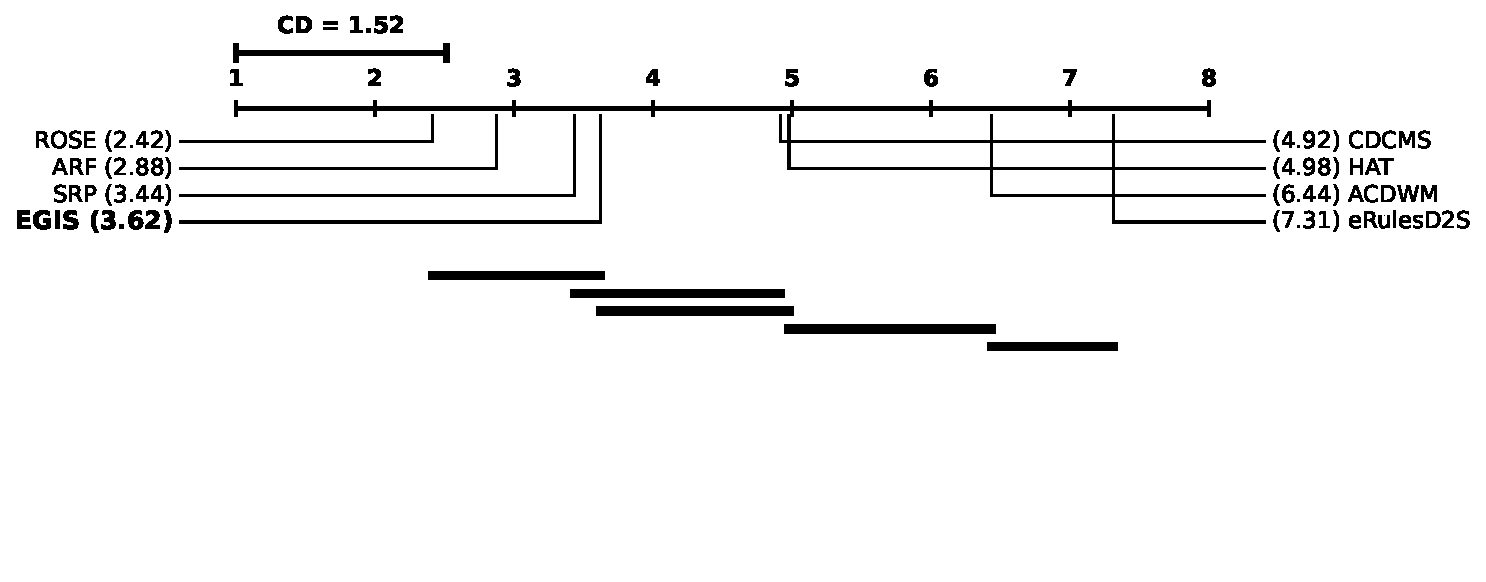
\includegraphics[width=0.95\textwidth]{figures/fig_critical_difference_all48.pdf}
\caption{Critical difference diagram for all 48 datasets (EXP-500-NP). Methods connected by a horizontal bar are not significantly different (Nemenyi, $\alpha = 0.05$).}
\label{fig:s_cd_all48}
\end{figure}

\subsection{Pairwise Wilcoxon Tests Across Configurations}
\label{sec:s3_pairwise}
Table~\ref{tab:s_pairwise_all} summarizes pairwise Wilcoxon tests (EGIS vs each baseline) across all configurations, including raw p-values, Bonferroni-adjusted p-values, and Cliff's delta effect sizes.

\begin{longtable}{llccccc}
\caption{Pairwise Wilcoxon Tests: EGIS vs Baselines (Binary Datasets)}\label{tab:s_pairwise_all} \\
\toprule
\textbf{Config} & \textbf{Comparison} & \textbf{Raw p} & \textbf{Adj. p} & \textbf{Sig.} & \textbf{$\delta$} & \textbf{Effect} \\
\midrule
\endfirsthead
\toprule
\textbf{Config} & \textbf{Comparison} & \textbf{Raw p} & \textbf{Adj. p} & \textbf{Sig.} & \textbf{$\delta$} & \textbf{Effect} \\
\midrule
\endhead
EXP-1000-NP & ARF & 0.1633 & 1.0000 & No & -0.133 & negligible \\
EXP-1000-NP & SRP & 0.8778 & 1.0000 & No & -0.055 & negligible \\
EXP-1000-NP & HAT & 0.0007 & 0.0052 & Yes & 0.197 & small \\
EXP-1000-NP & ROSE & $<$0.0001 & $<$0.0001 & Yes & -0.179 & small \\
EXP-1000-NP & ACDWM & $<$0.0001 & $<$0.0001 & Yes & 0.402 & medium \\
EXP-1000-NP & ERulesD2S & $<$0.0001 & $<$0.0001 & Yes & 0.926 & large \\
EXP-1000-NP & CDCMS & 0.0929 & 0.6505 & No & 0.084 & negligible \\
\midrule
EXP-2000-NP & ARF & 0.0437 & 0.3062 & No & -0.200 & small \\
EXP-2000-NP & SRP & 0.5811 & 1.0000 & No & -0.135 & negligible \\
EXP-2000-NP & HAT & 0.0061 & 0.0428 & Yes & 0.115 & negligible \\
EXP-2000-NP & ROSE & $<$0.0001 & 0.0002 & Yes & -0.248 & small \\
EXP-2000-NP & ACDWM & $<$0.0001 & $<$0.0001 & Yes & 0.611 & large \\
EXP-2000-NP & ERulesD2S & $<$0.0001 & $<$0.0001 & Yes & 0.930 & large \\
EXP-2000-NP & CDCMS & 0.2247 & 1.0000 & No & 0.002 & negligible \\
\midrule
EXP-500-NP & ARF & 0.0757 & 0.5298 & No & -0.172 & small \\
EXP-500-NP & SRP & 0.0825 & 0.5773 & No & -0.116 & negligible \\
EXP-500-NP & HAT & 0.0274 & 0.1921 & No & 0.180 & small \\
EXP-500-NP & ROSE & $<$0.0001 & 0.0006 & Yes & -0.184 & small \\
EXP-500-NP & ACDWM & 0.9535 & 1.0000 & No & 0.133 & negligible \\
EXP-500-NP & ERulesD2S & $<$0.0001 & $<$0.0001 & Yes & 0.843 & large \\
EXP-500-NP & CDCMS & 0.5908 & 1.0000 & No & 0.030 & negligible \\
\bottomrule
\end{longtable}


\section{Extended Transition Metrics}
\label{sec:s4}
This section provides detailed transition metric analysis across all seven EGIS configurations, extending the EXP-500-NP results presented in the main paper. Three metrics characterize rule set dynamics: Transition Change Score (TCS), Rule Identity Ratio (RIR), and Attribute Modification Score (AMS).

\subsection{Transition Metrics by Configuration}
\label{sec:s4_by_config}

\begin{longtable}{llccc}
\caption{Transition Metrics by Configuration and Drift Type}\label{tab:s_transitions_all} \\
\toprule
\textbf{Config} & \textbf{Drift Type} & \textbf{TCS} & \textbf{RIR} & \textbf{AMS} \\
\midrule
\endfirsthead
\toprule
\textbf{Config} & \textbf{Drift Type} & \textbf{TCS} & \textbf{RIR} & \textbf{AMS} \\
\midrule
\endhead
EXP-1000-NP & Abrupt & 0.236$\pm$0.113 & 0.252$\pm$0.202 & 0.285$\pm$0.091 \\
EXP-1000-NP & Gradual & 0.213$\pm$0.095 & 0.211$\pm$0.161 & 0.273$\pm$0.082 \\
EXP-1000-NP & Noisy & 0.226$\pm$0.092 & 0.218$\pm$0.167 & 0.301$\pm$0.063 \\
EXP-1000-NP & Stationary & 0.217$\pm$0.129 & 0.224$\pm$0.222 & 0.270$\pm$0.097 \\
EXP-1000-NP & Real & 0.221$\pm$0.092 & 0.226$\pm$0.160 & 0.265$\pm$0.062 \\
\midrule
EXP-1000-P & Abrupt & 0.236$\pm$0.112 & 0.251$\pm$0.204 & 0.284$\pm$0.091 \\
EXP-1000-P & Gradual & 0.217$\pm$0.097 & 0.218$\pm$0.164 & 0.275$\pm$0.083 \\
EXP-1000-P & Noisy & 0.227$\pm$0.090 & 0.220$\pm$0.161 & 0.300$\pm$0.062 \\
EXP-1000-P & Stationary & 0.219$\pm$0.131 & 0.231$\pm$0.226 & 0.268$\pm$0.095 \\
EXP-1000-P & Real & 0.214$\pm$0.092 & 0.211$\pm$0.162 & 0.268$\pm$0.062 \\
\midrule
EXP-2000-NP & Abrupt & 0.284$\pm$0.128 & 0.346$\pm$0.229 & 0.266$\pm$0.101 \\
EXP-2000-NP & Gradual & 0.233$\pm$0.128 & 0.243$\pm$0.228 & 0.275$\pm$0.073 \\
EXP-2000-NP & Noisy & 0.265$\pm$0.130 & 0.301$\pm$0.255 & 0.267$\pm$0.093 \\
EXP-2000-NP & Stationary & 0.171$\pm$0.096 & 0.147$\pm$0.144 & 0.255$\pm$0.099 \\
EXP-2000-NP & Real & 0.193$\pm$0.092 & 0.187$\pm$0.157 & 0.243$\pm$0.048 \\
\midrule
EXP-2000-P & Abrupt & 0.290$\pm$0.128 & 0.357$\pm$0.220 & 0.276$\pm$0.106 \\
EXP-2000-P & Gradual & 0.268$\pm$0.131 & 0.311$\pm$0.228 & 0.265$\pm$0.095 \\
EXP-2000-P & Noisy & 0.320$\pm$0.122 & 0.391$\pm$0.200 & 0.287$\pm$0.065 \\
EXP-2000-P & Stationary & 0.284$\pm$0.126 & 0.352$\pm$0.214 & 0.257$\pm$0.091 \\
EXP-2000-P & Real & 0.247$\pm$0.091 & 0.251$\pm$0.149 & 0.281$\pm$0.047 \\
\midrule
EXP-500-NP & Abrupt & 0.234$\pm$0.095 & 0.245$\pm$0.169 & 0.287$\pm$0.094 \\
EXP-500-NP & Gradual & 0.212$\pm$0.069 & 0.200$\pm$0.125 & 0.286$\pm$0.081 \\
EXP-500-NP & Noisy & 0.229$\pm$0.084 & 0.223$\pm$0.154 & 0.303$\pm$0.066 \\
EXP-500-NP & Stationary & 0.213$\pm$0.094 & 0.213$\pm$0.159 & 0.269$\pm$0.093 \\
EXP-500-NP & Real & 0.215$\pm$0.087 & 0.220$\pm$0.160 & 0.261$\pm$0.058 \\
\midrule
EXP-500-P & Abrupt & 0.230$\pm$0.100 & 0.239$\pm$0.166 & 0.288$\pm$0.097 \\
EXP-500-P & Gradual & 0.212$\pm$0.081 & 0.201$\pm$0.135 & 0.293$\pm$0.088 \\
EXP-500-P & Noisy & 0.229$\pm$0.077 & 0.219$\pm$0.145 & 0.304$\pm$0.061 \\
EXP-500-P & Stationary & 0.218$\pm$0.109 & 0.229$\pm$0.181 & 0.260$\pm$0.107 \\
EXP-500-P & Real & 0.209$\pm$0.070 & 0.203$\pm$0.122 & 0.265$\pm$0.057 \\
\midrule
EXP-500-P03 & Abrupt & 0.276$\pm$0.134 & 0.327$\pm$0.235 & 0.282$\pm$0.099 \\
EXP-500-P03 & Gradual & 0.265$\pm$0.130 & 0.301$\pm$0.234 & 0.286$\pm$0.082 \\
EXP-500-P03 & Noisy & 0.282$\pm$0.111 & 0.323$\pm$0.213 & 0.304$\pm$0.068 \\
EXP-500-P03 & Stationary & 0.267$\pm$0.137 & 0.321$\pm$0.236 & 0.263$\pm$0.102 \\
EXP-500-P03 & Real & 0.220$\pm$0.082 & 0.222$\pm$0.150 & 0.267$\pm$0.061 \\
\bottomrule
\end{longtable}

\subsection{TCS Distribution by Drift Type}
\label{sec:s4_tcs_violin}
\begin{figure*}[htbp]
\centering
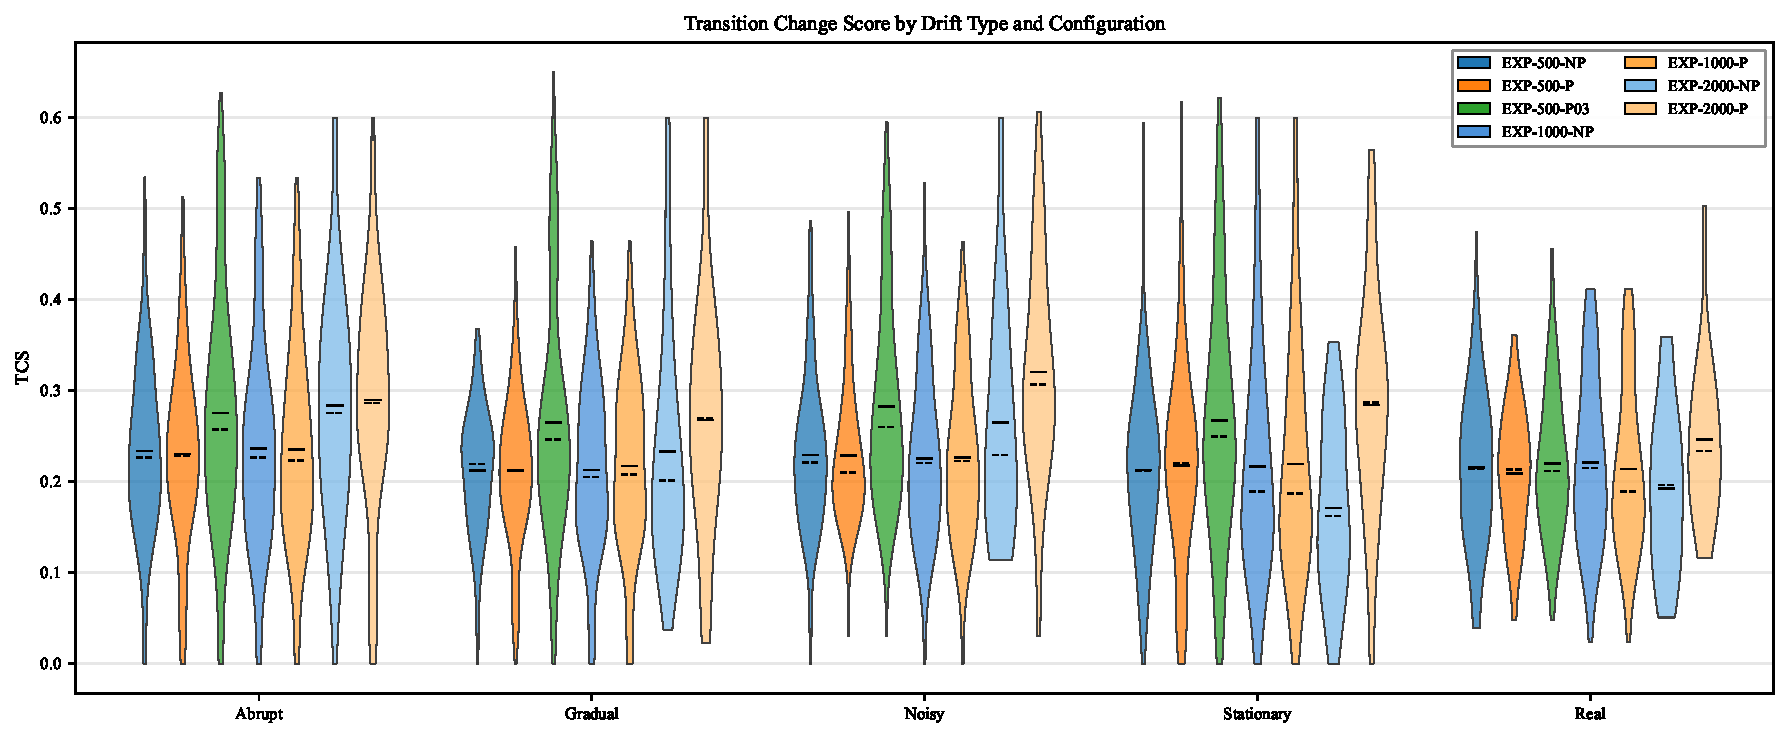
\includegraphics[width=0.95\textwidth]{figures/fig_violin_tcs.pdf}
\caption{Transition Change Score (TCS) distributions by drift type and EGIS configuration. Violin widths represent data density; horizontal bars indicate median values.}
\label{fig:s_violin_tcs}
\end{figure*}

Abrupt drift scenarios exhibit the highest TCS values (0.234$\pm$0.095 for EXP-500-NP), indicating substantial rule restructuring at drift points. Gradual drift shows lower TCS (0.212), suggesting smoother adaptation where the evolutionary process incrementally adjusts rules. Stationary streams maintain the lowest TCS (0.213), confirming minimal rule turnover when no concept change occurs. Noisy streams (0.229) and real-world streams (0.215) fall between these extremes.

Higher TCS in abrupt scenarios confirms that EGIS successfully detects and responds to sudden concept changes by substantially restructuring its rule set. The chunk size modulates this effect: larger chunks (EXP-1000-NP: 0.236; EXP-2000-NP: 0.284) yield progressively higher TCS for abrupt drift because fewer, more impactful transitions must absorb the same distributional shift. Penalty configurations show similar TCS patterns (EXP-500-P abrupt: 0.230, stationary: 0.218), indicating that the complexity penalty does not substantially alter the system's drift response dynamics.

\subsection{RIR Distribution by Drift Type}
\label{sec:s4_rir_violin}
\begin{figure*}[htbp]
\centering
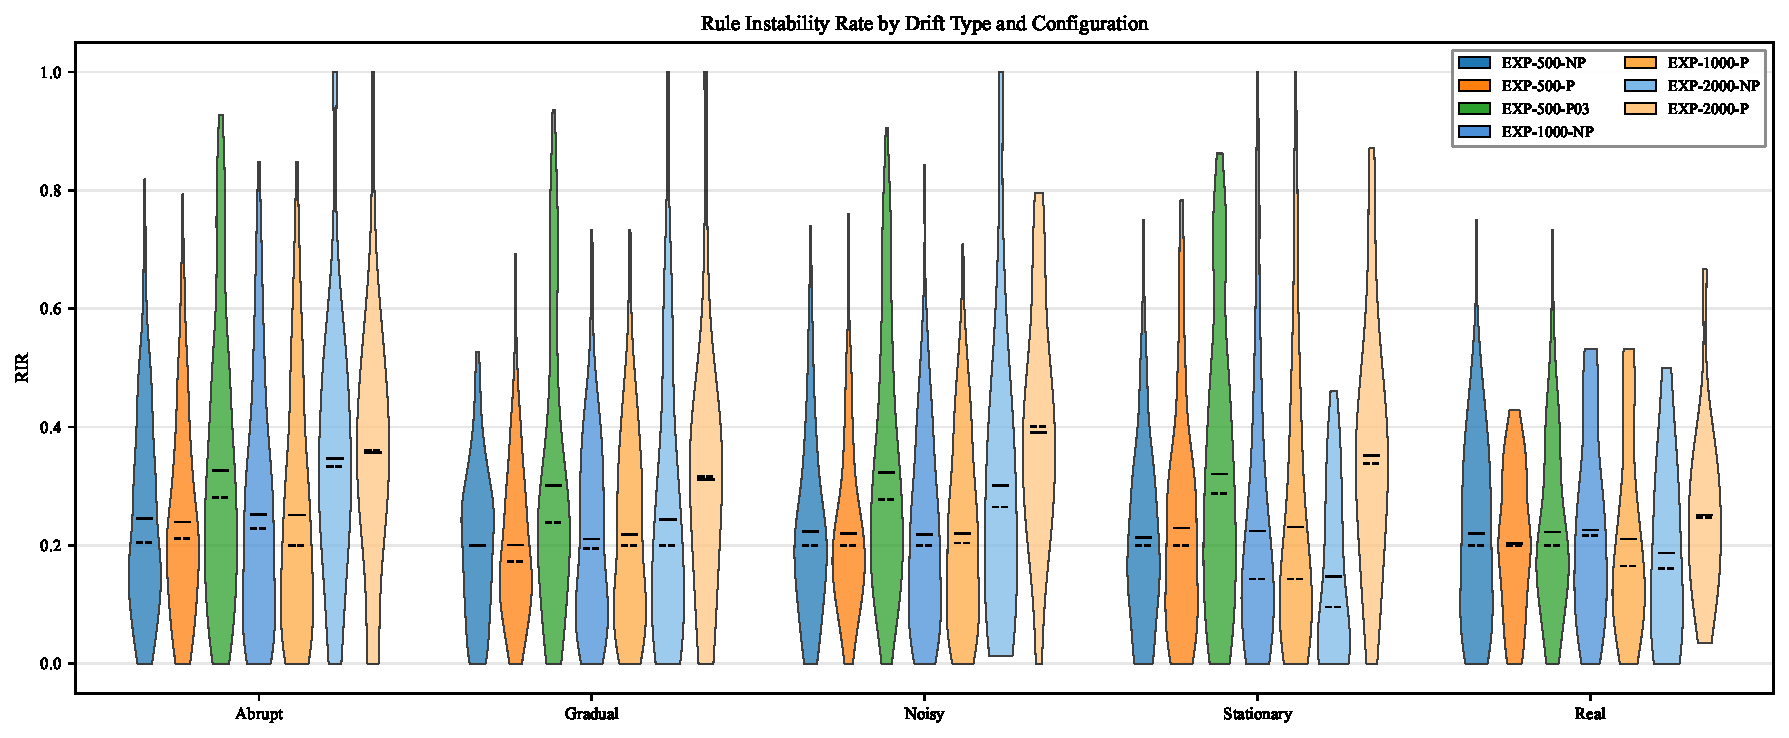
\includegraphics[width=0.95\textwidth]{figures/fig_violin_rir.pdf}
\caption{Rule Identity Ratio (RIR) distributions by drift type and EGIS configuration. Higher RIR values indicate greater structural change in rule identities across transitions.}
\label{fig:s_violin_rir}
\end{figure*}

The Rule Identity Ratio (RIR) captures the proportion of rules that are entirely replaced between consecutive chunks. Abrupt drift produces the highest RIR (0.245 for EXP-500-NP), consistent with the need to discard rules that become obsolete after a sudden concept shift. Gradual drift shows moderate RIR (0.200), while real-world streams exhibit the lowest (0.220), reflecting more conservative adaptation where the evolutionary process preserves useful rules.

While TCS captures overall change magnitude, RIR specifically measures complete rule replacement. The ratio TCS/RIR reveals the balance between rule modification and rule replacement: in stationary streams (RIR=0.213, TCS=0.213), most change comes from minor modifications rather than full replacements. Larger chunks (EXP-2000-NP abrupt RIR: 0.346) amplify rule replacement, as fewer evolutionary cycles must respond to the same magnitude of drift.

\subsection{AMS Distribution by Drift Type}
\label{sec:s4_ams_violin}
\begin{figure*}[htbp]
\centering
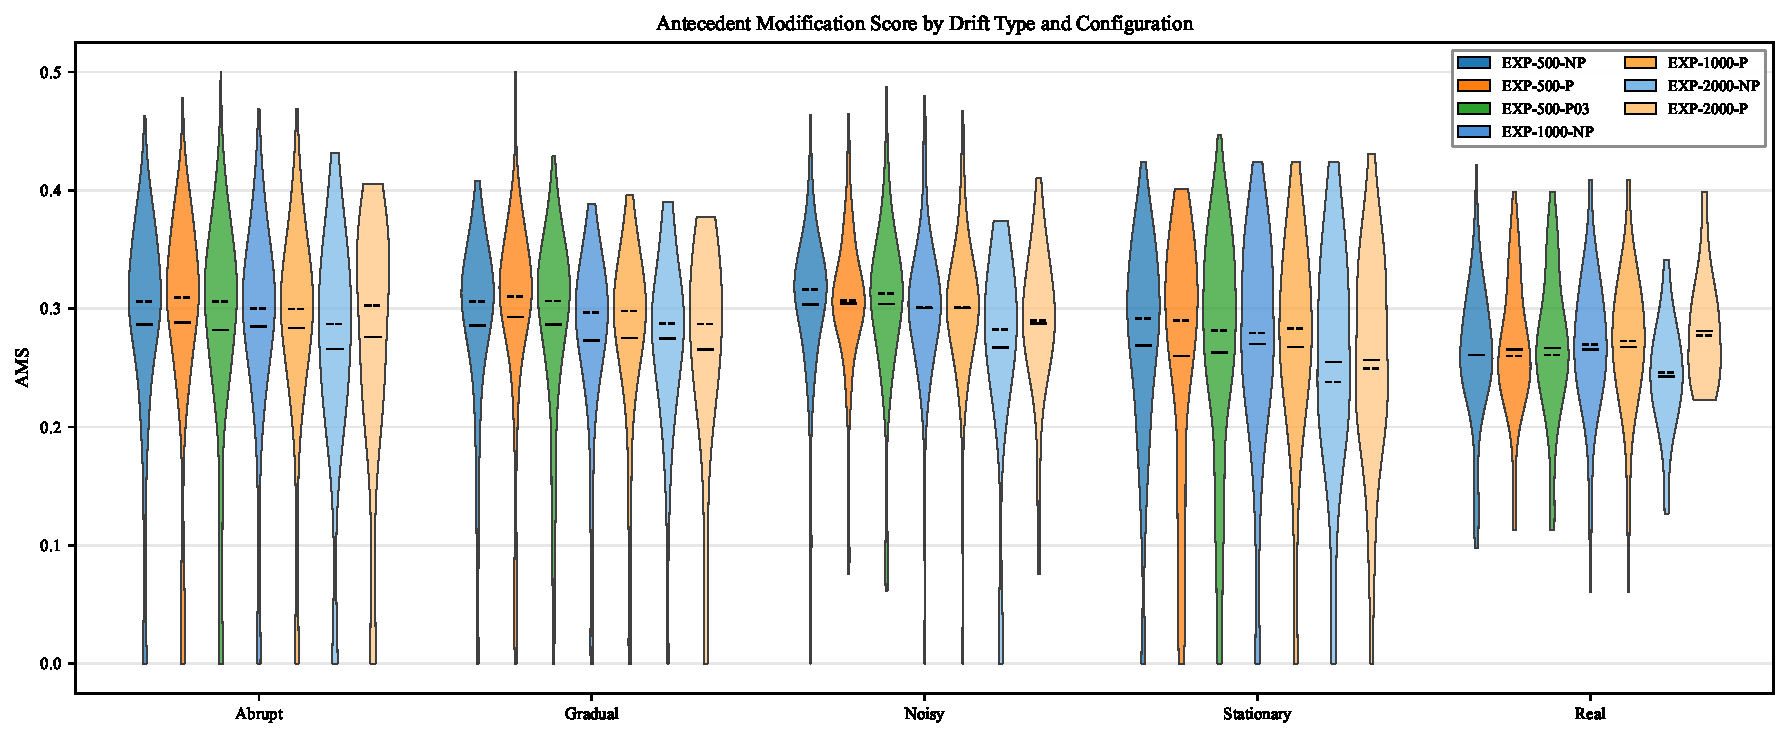
\includegraphics[width=0.95\textwidth]{figures/fig_violin_ams.pdf}
\caption{Attribute Modification Score (AMS) distributions by drift type and EGIS configuration. AMS measures how much the attribute usage pattern changes between consecutive rule sets.}
\label{fig:s_violin_ams}
\end{figure*}

The Attribute Modification Score (AMS) quantifies changes in feature usage across transitions. Abrupt drift exhibits the highest AMS (0.287), indicating significant shifts in which attributes the grammar selects. Noisy scenarios show moderate AMS (0.303), as noise induces some spurious attribute changes. Stationary streams show low AMS (0.269), confirming stable feature selection when the underlying concept remains unchanged.

Low AMS in stationary streams suggests that EGIS maintains consistent feature selection when the data distribution is stable, an important property for interpretability: practitioners can trust that the selected features reflect genuine data patterns rather than evolutionary noise. Gradual drift (0.286) and real-world streams (0.261) show intermediate AMS, consistent with their more moderate distributional shifts.

\subsection{Transition Metrics Synthesis}
\label{sec:s4_synthesis}
Taken together, the three transition metrics paint a coherent picture of EGIS's adaptive behavior. In abrupt drift, all three metrics peak (TCS=0.234, RIR=0.245, AMS=0.287), confirming that the evolutionary process responds to sudden shifts through comprehensive rule restructuring: replacing rules (high RIR), changing feature usage (high AMS), and achieving high overall change (high TCS). In stationary settings, all three metrics are low (TCS=0.213, RIR=0.213, AMS=0.269), demonstrating that EGIS avoids unnecessary rule churn when no drift occurs. This drift-proportional response validates the custom severity classification mechanism, which governs how aggressively the evolutionary process explores new rule structures.


\section{EGIS Configuration Analysis}
\label{sec:s5}
This section analyzes how EGIS performance varies across chunk size and complexity penalty configurations. Results are based on the 41 binary datasets.

\subsection{Chunk Size Effect}
\label{sec:s5_chunk}
\begin{figure*}[htbp]
\centering
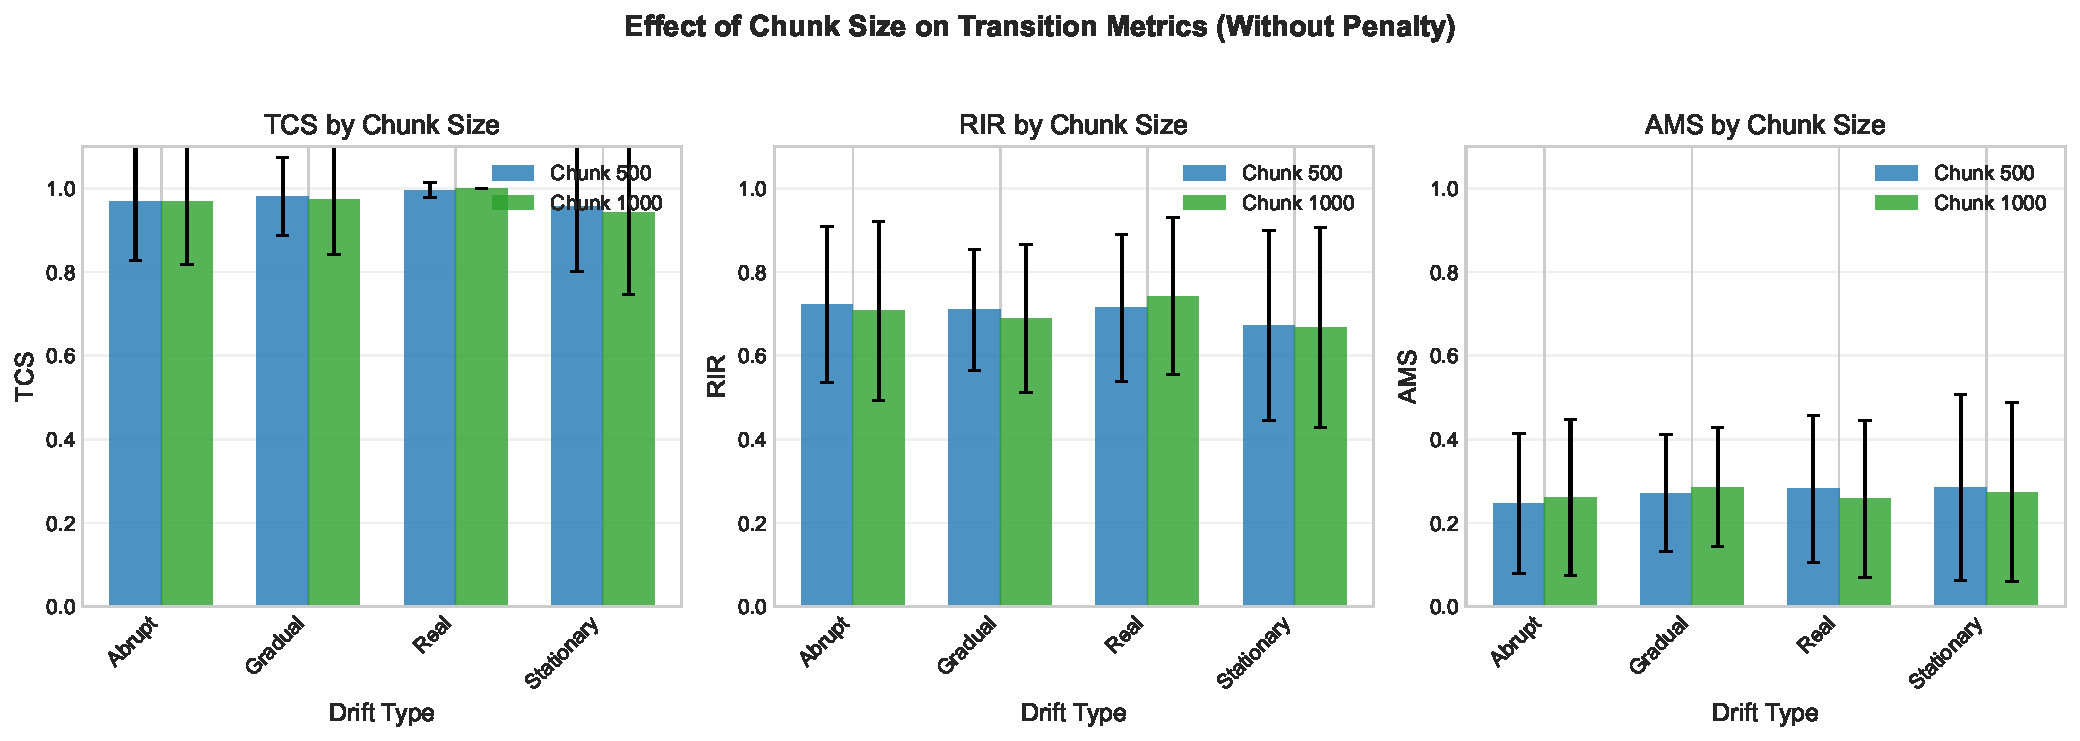
\includegraphics[width=0.95\textwidth]{figures/fig_chunk_size_effect.pdf}
\caption{Chunk size sensitivity analysis showing EGIS performance (G-Mean) across no-penalty configurations for each drift type.}
\label{fig:s_chunk_size}
\end{figure*}

EXP-500-NP achieves a mean G-Mean of 0.859 on binary datasets. Increasing the chunk size to 1000 yields 0.869 (+1.0pp), while chunk size 2000 produces 0.855 (-0.4pp). These configurations provide 23, 11, and 5 evolutionary transitions respectively (the first chunk initializes the model).

\begin{table}[htbp]
\centering
\caption{EGIS Mean G-Mean by Chunk Size and Drift Type}
\label{tab:s5_chunk_drift}
\footnotesize
\begin{tabular}{lccc}
\toprule
\textbf{Drift Type} & \textbf{EXP-500-NP} & \textbf{EXP-1000-NP} & \textbf{EXP-2000-NP} \\
\midrule
Abrupt & 0.860 & \textbf{0.868} & 0.837 \\
Gradual & 0.855 & \textbf{0.867} & 0.858 \\
Noisy & 0.846 & \textbf{0.851} & 0.836 \\
Stationary & 0.862 & 0.873 & \textbf{0.881} \\
Real-world & 0.890 & \textbf{0.912} & 0.908 \\
\bottomrule
\end{tabular}
\end{table}

The optimal chunk size varies by drift type (Table~\ref{tab:s5_chunk_drift}): EXP-1000-NP performs best on abrupt drift, EXP-1000-NP on gradual drift, and EXP-2000-NP on stationary scenarios. Smaller chunks (23 transitions) enable finer-grained evolutionary adaptation to sudden changes, while larger chunks (5 transitions) provide more training data per evolutionary cycle, benefiting stable or slowly evolving distributions. This trade-off between adaptation granularity and training sample size is a key design consideration for grammar-based stream classifiers.

\subsection{Complexity Penalty Effect}
\label{sec:s5_penalty}
\begin{figure*}[htbp]
\centering
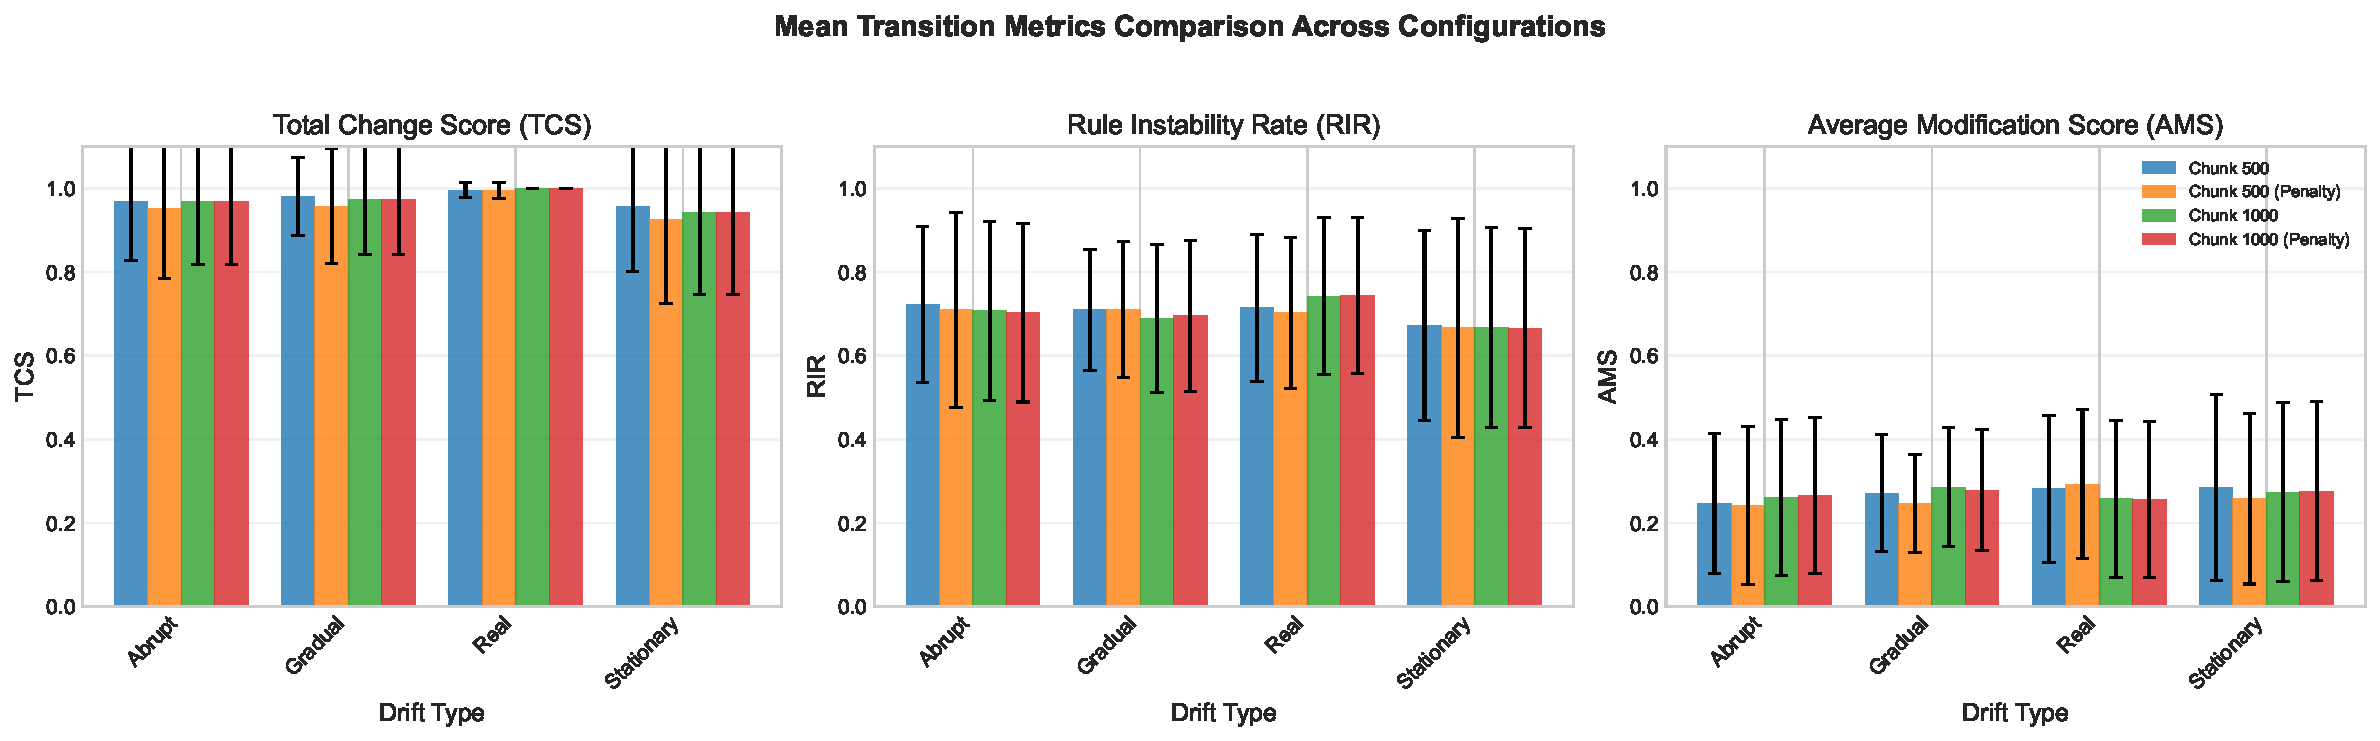
\includegraphics[width=0.95\textwidth]{figures/fig_config_comparison.pdf}
\caption{Configuration comparison showing the combined effect of chunk size and complexity penalty on EGIS performance across all binary datasets.}
\label{fig:s_config_comp}
\end{figure*}

The complexity penalty ($\gamma$) trades classification accuracy for simpler, more interpretable rules. At $\gamma=0.1$, EXP-500-P achieves 0.860 (+0.0pp vs NP), showing minimal impact. At $\gamma=0.3$, EXP-500-P03 yields 0.846 (-1.3pp), a more noticeable degradation that reflects the stronger pressure toward simpler rule sets. This pattern holds across chunk sizes: EXP-1000-P achieves 0.869 (-0.0pp vs NP) and EXP-2000-P achieves 0.851 (-0.4pp vs NP).

The penalty impact varies by drift type (EXP-500-P vs EXP-500-NP): abrupt (+0.3pp); gradual (+0.1pp); noisy (-0.4pp); stationary (+0.1pp); real (-0.1pp). 
In terms of interpretability, the penalty reduces mean rule complexity from 5.3 to 4.6 conditions per rule (13\% reduction), producing more compact and human-readable models at a modest accuracy cost.

\subsection{Performance by Drift Type}
\label{sec:s5_drift}
\begin{figure}[htbp]
\centering
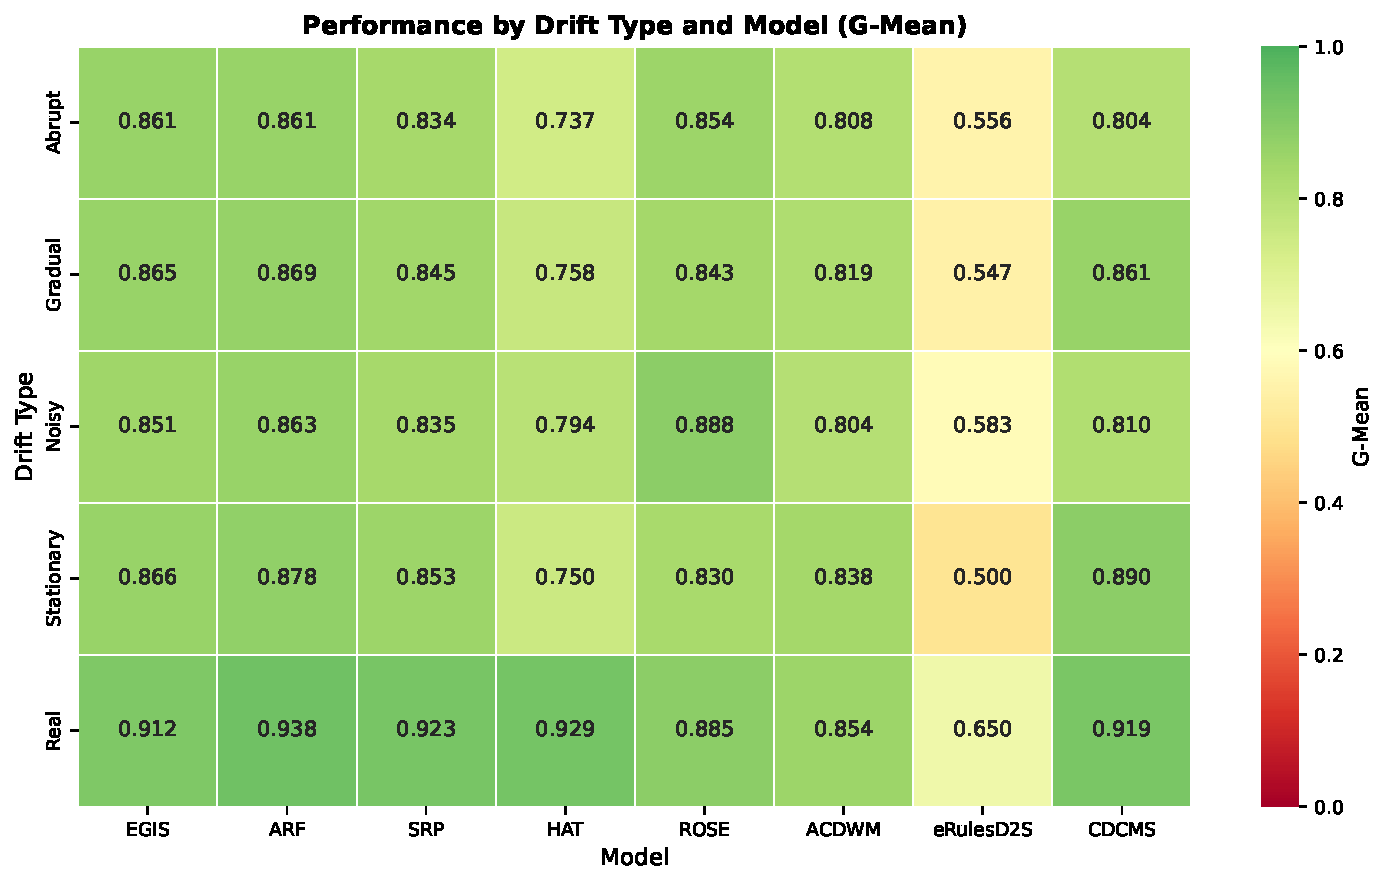
\includegraphics[width=0.95\columnwidth]{figures/fig7_drift_heatmap.pdf}
\caption{Performance heatmap: mean G-Mean by model and drift type (EXP-500-NP, binary datasets). Darker shading indicates higher performance.}
\label{fig:s_heatmap}
\end{figure}

\begin{figure*}[htbp]
\centering
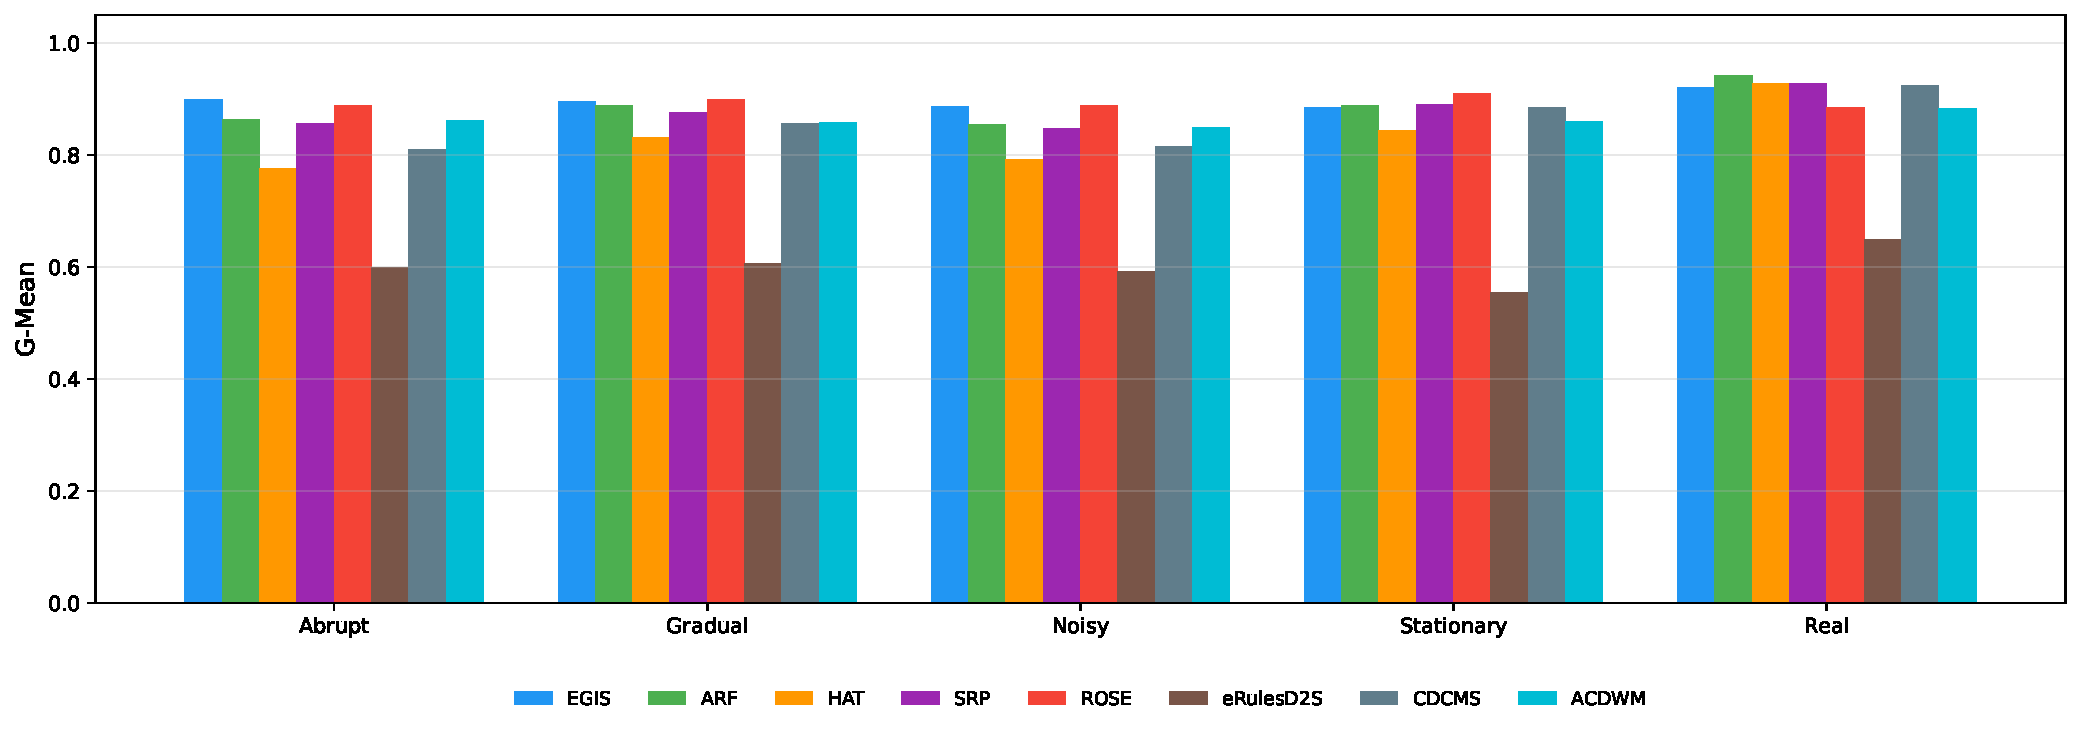
\includegraphics[width=0.95\textwidth]{figures/fig_metrics_by_drift.pdf}
\caption{Performance comparison by drift type showing G-Mean for each model across drift categories (EXP-500-NP, binary datasets).}
\label{fig:s_metrics_drift}
\end{figure*}

\begin{table}[htbp]
\centering
\caption{EGIS Performance by Drift Type vs Top Models (EXP-500-NP)}
\label{tab:s5_drift_ranking}
\footnotesize
\begin{tabular}{lcccccc}
\toprule
\textbf{Drift Type} & \textbf{EGIS} & \textbf{Rank} & \textbf{ARF} & \textbf{ROSE} & \textbf{SRP} & \textbf{Best} \\
\midrule
Abrupt & 0.860 & 4/8 & 0.863 & 0.888 & 0.857 & ROSE \\
Gradual & 0.855 & 6/8 & 0.888 & 0.900 & 0.875 & ROSE \\
Noisy & 0.846 & 5/8 & 0.855 & 0.888 & 0.847 & ROSE \\
Stationary & 0.862 & 5/8 & 0.883 & 0.901 & 0.877 & ROSE \\
Real-world & 0.890 & 5/8 & 0.941 & 0.885 & 0.929 & ARF \\
\bottomrule
\end{tabular}
\end{table}

Table~\ref{tab:s5_drift_ranking} and the figures above reveal how EGIS performs relative to baselines across drift types (EXP-500-NP). Per drift type, EGIS achieves: abrupt (0.860, rank 4/8, best: ROSE 0.888); gradual (0.855, rank 6/8, best: ROSE 0.900); noisy (0.846, rank 5/8, best: ROSE 0.888); stationary (0.862, rank 5/8, best: ROSE 0.901); real-world (0.890, rank 5/8, best: ARF 0.941). 
EGIS performs best on real-world scenarios (0.890) and shows more difficulty with noisy drift (0.846). 

EGIS is most competitive (top-4 rank) on abrupt scenarios. 
On gradual, noisy, stationary, real-world scenarios, EGIS ranks lower, with a 4.3pp gap to the best model on noisy drift. This may reflect the inherent difficulty of evolving rule sets for these scenarios, where ensemble methods with built-in drift detectors can adapt more rapidly through their constituent learner replacement mechanisms.

\subsection{Drift Detection Summary}
\label{sec:s5_drift_detect}
Table~\ref{tab:s5_drift_detect} summarizes drift detection frequency across EGIS configurations. Drift events are identified by the custom severity classification mechanism described in Section~\ref{sec:s1_params}.

\begin{table}[htbp]
\centering
\caption{Drift Detection Frequency by Configuration}
\label{tab:s5_drift_detect}
\footnotesize
\begin{tabular}{lcc}
\toprule
\textbf{Config} & \textbf{Avg Drifts/Dataset} & \textbf{Max Drifts} \\
\midrule
EXP-500-NP & 1.19 & 7 \\
EXP-500-P & 1.10 & 7 \\
EXP-500-P03 & 2.42 & 11 \\
EXP-1000-NP & 0.69 & 3 \\
EXP-1000-P & 0.67 & 3 \\
EXP-2000-NP & 0.42 & 2 \\
EXP-2000-P & 0.54 & 2 \\
\bottomrule
\end{tabular}
\end{table}

Drift detection frequency decreases with chunk size: EXP-500 configurations detect an average of 1.10--2.42 drifts per dataset, while EXP-2000 configurations detect only 0.42--0.54. This is expected because larger chunks smooth out distributional shifts, making abrupt changes less distinguishable from the overall data distribution within each chunk. The penalty factor ($\gamma=0.3$) substantially increases detection frequency (EXP-500-P03: 2.42 vs EXP-500-NP: 1.19), because the complexity penalty creates evolutionary pressure to restructure the rule set, which the severity classifier interprets as concept change.


\section{Per-Dataset Visual Analysis}
\label{sec:s6}
This section presents case study visualizations for each of the 48 datasets using the primary configuration EXP-500-NP. Each composite 2$\times$2 figure shows: (a) accuracy over time with detected drifts, (b) rule evolution counts (stacked area), (c) rule complexity (dual-axis), and (d) transition metrics (TCS, RIR, AMS). Equivalent figures for EXP-1000-NP and EXP-2000-NP are available in the accompanying digital archive.

\subsection{Abrupt Drift Datasets}
\label{sec:s6_abrupt}

\subsubsection{AGRAWAL\_Abrupt\_Chain\_Long}
\begin{figure}[htbp]
\centering

\includegraphics[width=0.95\textwidth,height=0.42\textheight,keepaspectratio]{figures/case_studies/EXP-500-NP/AGRAWAL_Abrupt_Chain_Long.pdf}
\caption{Case study: AGRAWAL\_Abrupt\_Chain\_Long (Abrupt drift, EXP-500-NP). Panels show (a) accuracy with detected drifts, (b) rule evolution counts, (c) rule complexity, and (d) transition metrics.}
\label{fig:s6_agrawal_abrupt_chain_long}
\end{figure}

On AGRAWAL\_Abrupt\_Chain\_Long (Abrupt), EGIS achieves the best G-Mean of 0.888 among 8 models, demonstrating its effectiveness on this Abrupt scenario. Specifically, EGIS outperforms ARF by 10.0pp, outperforms ROSE by 5.8pp, outperforms SRP by 10.3pp. The moderate TCS of 0.29 (RIR=0.35, AMS=0.32) is consistent with the need for rapid rule restructuring in response to sudden concept changes.

\vspace{0.5cm}

\subsubsection{AGRAWAL\_Abrupt\_Simple\_Mild}
\begin{figure}[htbp]
\centering

\includegraphics[width=0.95\textwidth,height=0.42\textheight,keepaspectratio]{figures/case_studies/EXP-500-NP/AGRAWAL_Abrupt_Simple_Mild.pdf}
\caption{Case study: AGRAWAL\_Abrupt\_Simple\_Mild (Abrupt drift, EXP-500-NP). Panels show (a) accuracy with detected drifts, (b) rule evolution counts, (c) rule complexity, and (d) transition metrics.}
\label{fig:s6_agrawal_abrupt_simple_mild}
\end{figure}

On AGRAWAL\_Abrupt\_Simple\_Mild (Abrupt), EGIS achieves the best G-Mean of 0.906 among 8 models, demonstrating its effectiveness on this Abrupt scenario. Specifically, EGIS outperforms ARF by 8.1pp, outperforms ROSE by 0.5pp, outperforms SRP by 3.9pp. The moderate TCS of 0.34 (RIR=0.43, AMS=0.36) is consistent with the need for rapid rule restructuring in response to sudden concept changes.

\clearpage

\subsubsection{AGRAWAL\_Abrupt\_Simple\_Severe}
\begin{figure}[htbp]
\centering

\includegraphics[width=0.95\textwidth,height=0.42\textheight,keepaspectratio]{figures/case_studies/EXP-500-NP/AGRAWAL_Abrupt_Simple_Severe.pdf}
\caption{Case study: AGRAWAL\_Abrupt\_Simple\_Severe (Abrupt drift, EXP-500-NP). Panels show (a) accuracy with detected drifts, (b) rule evolution counts, (c) rule complexity, and (d) transition metrics.}
\label{fig:s6_agrawal_abrupt_simple_severe}
\end{figure}

On AGRAWAL\_Abrupt\_Simple\_Severe (Abrupt), EGIS achieves a G-Mean of 0.900, ranking 2/8 (2.5pp behind ROSE at 0.925). Specifically, EGIS outperforms ARF by 6.0pp, trails ROSE by 2.5pp, outperforms SRP by 1.0pp. The high TCS of 0.35 (RIR=0.45, AMS=0.36) is consistent with the need for rapid rule restructuring in response to sudden concept changes.

\vspace{0.5cm}

\subsubsection{HYPERPLANE\_Abrupt\_Simple}
\begin{figure}[htbp]
\centering

\includegraphics[width=0.95\textwidth,height=0.42\textheight,keepaspectratio]{figures/case_studies/EXP-500-NP/HYPERPLANE_Abrupt_Simple.pdf}
\caption{Case study: HYPERPLANE\_Abrupt\_Simple (Abrupt drift, EXP-500-NP). Panels show (a) accuracy with detected drifts, (b) rule evolution counts, (c) rule complexity, and (d) transition metrics.}
\label{fig:s6_hyperplane_abrupt_simple}
\end{figure}

On HYPERPLANE\_Abrupt\_Simple (Abrupt), EGIS achieves a G-Mean of 0.756, ranking 7/8 (14.8pp behind CDCMS at 0.904). Specifically, EGIS trails ARF by 8.0pp, trails ROSE by 10.8pp, trails SRP by 1.6pp. The moderate TCS of 0.20 (RIR=0.16, AMS=0.30) is consistent with the need for rapid rule restructuring in response to sudden concept changes.

\clearpage

\subsubsection{LED\_Abrupt\_Simple}
\begin{figure}[htbp]
\centering

\includegraphics[width=0.95\textwidth,height=0.42\textheight,keepaspectratio]{figures/case_studies/EXP-500-NP/LED_Abrupt_Simple.pdf}
\caption{Case study: LED\_Abrupt\_Simple (Abrupt drift, EXP-500-NP). Panels show (a) accuracy with detected drifts, (b) rule evolution counts, (c) rule complexity, and (d) transition metrics.}
\label{fig:s6_led_abrupt_simple}
\end{figure}

On LED\_Abrupt\_Simple (Abrupt), EGIS achieves the best G-Mean of 0.908 among 6 models, demonstrating its effectiveness on this Abrupt scenario. Specifically, EGIS outperforms ARF by 7.8pp, outperforms ROSE by 50.3pp, outperforms SRP by 32.9pp. The low TCS of 0.10 (RIR=0.09, AMS=0.14) is consistent with the need for rapid rule restructuring in response to sudden concept changes.

\vspace{0.5cm}

\subsubsection{RANDOMTREE\_Abrupt\_Recurring}
\begin{figure}[htbp]
\centering

\includegraphics[width=0.95\textwidth,height=0.42\textheight,keepaspectratio]{figures/case_studies/EXP-500-NP/RANDOMTREE_Abrupt_Recurring.pdf}
\caption{Case study: RANDOMTREE\_Abrupt\_Recurring (Abrupt drift, EXP-500-NP). Panels show (a) accuracy with detected drifts, (b) rule evolution counts, (c) rule complexity, and (d) transition metrics.}
\label{fig:s6_randomtree_abrupt_recurring}
\end{figure}

On RANDOMTREE\_Abrupt\_Recurring (Abrupt), EGIS achieves a G-Mean of 0.615, ranking 3/8 (7.0pp behind ACDWM at 0.685). Specifically, EGIS outperforms ARF by 8.2pp, trails ROSE by 3.9pp, outperforms SRP by 9.1pp. The moderate TCS of 0.26 (RIR=0.29, AMS=0.28) is consistent with the need for rapid rule restructuring in response to sudden concept changes.

\clearpage

\subsubsection{RANDOMTREE\_Abrupt\_Simple}
\begin{figure}[htbp]
\centering

\includegraphics[width=0.95\textwidth,height=0.42\textheight,keepaspectratio]{figures/case_studies/EXP-500-NP/RANDOMTREE_Abrupt_Simple.pdf}
\caption{Case study: RANDOMTREE\_Abrupt\_Simple (Abrupt drift, EXP-500-NP). Panels show (a) accuracy with detected drifts, (b) rule evolution counts, (c) rule complexity, and (d) transition metrics.}
\label{fig:s6_randomtree_abrupt_simple}
\end{figure}

On RANDOMTREE\_Abrupt\_Simple (Abrupt), EGIS achieves a G-Mean of 0.614, ranking 3/8 (7.0pp behind ACDWM at 0.684). Specifically, EGIS outperforms ARF by 6.4pp, trails ROSE by 4.6pp, outperforms SRP by 10.3pp. The moderate TCS of 0.26 (RIR=0.30, AMS=0.28) is consistent with the need for rapid rule restructuring in response to sudden concept changes.

\vspace{0.5cm}

\subsubsection{RBF\_Abrupt\_Blip}
\begin{figure}[htbp]
\centering

\includegraphics[width=0.95\textwidth,height=0.42\textheight,keepaspectratio]{figures/case_studies/EXP-500-NP/RBF_Abrupt_Blip.pdf}
\caption{Case study: RBF\_Abrupt\_Blip (Abrupt drift, EXP-500-NP). Panels show (a) accuracy with detected drifts, (b) rule evolution counts, (c) rule complexity, and (d) transition metrics.}
\label{fig:s6_rbf_abrupt_blip}
\end{figure}

On RBF\_Abrupt\_Blip (Abrupt), EGIS achieves a G-Mean of 0.832, ranking 7/8 (8.4pp behind SRP at 0.916). Specifically, EGIS trails ARF by 7.8pp, trails ROSE by 6.4pp, trails SRP by 8.4pp. The moderate TCS of 0.24 (RIR=0.23, AMS=0.32) is consistent with the need for rapid rule restructuring in response to sudden concept changes.

\clearpage

\subsubsection{RBF\_Abrupt\_Severe}
\begin{figure}[htbp]
\centering

\includegraphics[width=0.95\textwidth,height=0.42\textheight,keepaspectratio]{figures/case_studies/EXP-500-NP/RBF_Abrupt_Severe.pdf}
\caption{Case study: RBF\_Abrupt\_Severe (Abrupt drift, EXP-500-NP). Panels show (a) accuracy with detected drifts, (b) rule evolution counts, (c) rule complexity, and (d) transition metrics.}
\label{fig:s6_rbf_abrupt_severe}
\end{figure}

On RBF\_Abrupt\_Severe (Abrupt), EGIS achieves a G-Mean of 0.807, ranking 5/8 (9.5pp behind SRP at 0.901). Specifically, EGIS trails ARF by 8.7pp, trails ROSE by 6.3pp, trails SRP by 9.5pp. The moderate TCS of 0.25 (RIR=0.25, AMS=0.33) is consistent with the need for rapid rule restructuring in response to sudden concept changes.

\vspace{0.5cm}

\subsubsection{SEA\_Abrupt\_Chain}
\begin{figure}[htbp]
\centering

\includegraphics[width=0.95\textwidth,height=0.42\textheight,keepaspectratio]{figures/case_studies/EXP-500-NP/SEA_Abrupt_Chain.pdf}
\caption{Case study: SEA\_Abrupt\_Chain (Abrupt drift, EXP-500-NP). Panels show (a) accuracy with detected drifts, (b) rule evolution counts, (c) rule complexity, and (d) transition metrics.}
\label{fig:s6_sea_abrupt_chain}
\end{figure}

On SEA\_Abrupt\_Chain (Abrupt), EGIS achieves a G-Mean of 0.947, ranking 4/8 (3.0pp behind ROSE at 0.977). Specifically, EGIS trails ARF by 2.5pp, trails ROSE by 3.0pp, trails SRP by 0.9pp. The low TCS of 0.18 (RIR=0.13, AMS=0.31) is consistent with the need for rapid rule restructuring in response to sudden concept changes.

\clearpage

\subsubsection{SEA\_Abrupt\_Recurring}
\begin{figure}[htbp]
\centering

\includegraphics[width=0.95\textwidth,height=0.42\textheight,keepaspectratio]{figures/case_studies/EXP-500-NP/SEA_Abrupt_Recurring.pdf}
\caption{Case study: SEA\_Abrupt\_Recurring (Abrupt drift, EXP-500-NP). Panels show (a) accuracy with detected drifts, (b) rule evolution counts, (c) rule complexity, and (d) transition metrics.}
\label{fig:s6_sea_abrupt_recurring}
\end{figure}

On SEA\_Abrupt\_Recurring (Abrupt), EGIS achieves a G-Mean of 0.945, ranking 5/8 (3.2pp behind ARF at 0.977). Specifically, EGIS trails ARF by 3.2pp, trails ROSE by 3.0pp, outperforms SRP by 0.6pp. The moderate TCS of 0.22 (RIR=0.19, AMS=0.31) is consistent with the need for rapid rule restructuring in response to sudden concept changes.

\vspace{0.5cm}

\subsubsection{SEA\_Abrupt\_Simple}
\begin{figure}[htbp]
\centering

\includegraphics[width=0.95\textwidth,height=0.42\textheight,keepaspectratio]{figures/case_studies/EXP-500-NP/SEA_Abrupt_Simple.pdf}
\caption{Case study: SEA\_Abrupt\_Simple (Abrupt drift, EXP-500-NP). Panels show (a) accuracy with detected drifts, (b) rule evolution counts, (c) rule complexity, and (d) transition metrics.}
\label{fig:s6_sea_abrupt_simple}
\end{figure}

On SEA\_Abrupt\_Simple (Abrupt), EGIS achieves a G-Mean of 0.950, ranking 5/8 (2.9pp behind ROSE at 0.979). Specifically, EGIS trails ARF by 2.8pp, trails ROSE by 2.9pp, trails SRP by 2.4pp. The moderate TCS of 0.20 (RIR=0.16, AMS=0.32) is consistent with the need for rapid rule restructuring in response to sudden concept changes.

\clearpage

\subsubsection{SINE\_Abrupt\_Simple}
\begin{figure}[htbp]
\centering

\includegraphics[width=0.95\textwidth,height=0.42\textheight,keepaspectratio]{figures/case_studies/EXP-500-NP/SINE_Abrupt_Simple.pdf}
\caption{Case study: SINE\_Abrupt\_Simple (Abrupt drift, EXP-500-NP). Panels show (a) accuracy with detected drifts, (b) rule evolution counts, (c) rule complexity, and (d) transition metrics.}
\label{fig:s6_sine_abrupt_simple}
\end{figure}

On SINE\_Abrupt\_Simple (Abrupt), EGIS achieves a G-Mean of 0.951, ranking 6/8 (3.7pp behind ARF at 0.988). Specifically, EGIS trails ARF by 3.7pp, trails ROSE by 2.9pp, trails SRP by 3.6pp. The low TCS of 0.15 (RIR=0.09, AMS=0.25) is consistent with the need for rapid rule restructuring in response to sudden concept changes.

\vspace{0.5cm}

\subsubsection{STAGGER\_Abrupt\_Chain}
\begin{figure}[htbp]
\centering

\includegraphics[width=0.95\textwidth,height=0.42\textheight,keepaspectratio]{figures/case_studies/EXP-500-NP/STAGGER_Abrupt_Chain.pdf}
\caption{Case study: STAGGER\_Abrupt\_Chain (Abrupt drift, EXP-500-NP). Panels show (a) accuracy with detected drifts, (b) rule evolution counts, (c) rule complexity, and (d) transition metrics.}
\label{fig:s6_stagger_abrupt_chain}
\end{figure}

On STAGGER\_Abrupt\_Chain (Abrupt), EGIS achieves a G-Mean of 0.968, ranking 4/8 (2.7pp behind ARF at 0.994). Specifically, EGIS trails ARF by 2.7pp, outperforms ROSE by 4.6pp, trails SRP by 2.5pp. The moderate TCS of 0.22 (RIR=0.29, AMS=0.18) is consistent with the need for rapid rule restructuring in response to sudden concept changes.

\clearpage

\subsubsection{STAGGER\_Abrupt\_Recurring}
\begin{figure}[htbp]
\centering

\includegraphics[width=0.95\textwidth,height=0.42\textheight,keepaspectratio]{figures/case_studies/EXP-500-NP/STAGGER_Abrupt_Recurring.pdf}
\caption{Case study: STAGGER\_Abrupt\_Recurring (Abrupt drift, EXP-500-NP). Panels show (a) accuracy with detected drifts, (b) rule evolution counts, (c) rule complexity, and (d) transition metrics.}
\label{fig:s6_stagger_abrupt_recurring}
\end{figure}

On STAGGER\_Abrupt\_Recurring (Abrupt), EGIS achieves a G-Mean of 0.957, ranking 5/8 (4.1pp behind ROSE at 0.997). Specifically, EGIS trails ARF by 4.0pp, trails ROSE by 4.1pp, trails SRP by 3.2pp. The moderate TCS of 0.22 (RIR=0.30, AMS=0.15) is consistent with the need for rapid rule restructuring in response to sudden concept changes.

\vspace{0.5cm}

\subsubsection{WAVEFORM\_Abrupt\_Simple}
\begin{figure}[htbp]
\centering

\includegraphics[width=0.95\textwidth,height=0.42\textheight,keepaspectratio]{figures/case_studies/EXP-500-NP/WAVEFORM_Abrupt_Simple.pdf}
\caption{Case study: WAVEFORM\_Abrupt\_Simple (Abrupt drift, EXP-500-NP). Panels show (a) accuracy with detected drifts, (b) rule evolution counts, (c) rule complexity, and (d) transition metrics.}
\label{fig:s6_waveform_abrupt_simple}
\end{figure}

On WAVEFORM\_Abrupt\_Simple (Abrupt), EGIS achieves a G-Mean of 0.722, ranking 5/6 (10.2pp behind ROSE at 0.824). Specifically, EGIS trails ARF by 7.3pp, trails ROSE by 10.2pp, trails SRP by 9.7pp. The moderate TCS of 0.24 (RIR=0.21, AMS=0.37) is consistent with the need for rapid rule restructuring in response to sudden concept changes.

\clearpage

\subsection{Gradual Drift Datasets}
\label{sec:s6_gradual}

\subsubsection{HYPERPLANE\_Gradual\_Simple}
\begin{figure}[htbp]
\centering

\includegraphics[width=0.95\textwidth,height=0.42\textheight,keepaspectratio]{figures/case_studies/EXP-500-NP/HYPERPLANE_Gradual_Simple.pdf}
\caption{Case study: HYPERPLANE\_Gradual\_Simple (Gradual drift, EXP-500-NP). Panels show (a) accuracy with detected drifts, (b) rule evolution counts, (c) rule complexity, and (d) transition metrics.}
\label{fig:s6_hyperplane_gradual_simple}
\end{figure}

On HYPERPLANE\_Gradual\_Simple (Gradual), EGIS achieves a G-Mean of 0.756, ranking 7/8 (14.8pp behind CDCMS at 0.904). Specifically, EGIS trails ARF by 7.6pp, trails ROSE by 10.8pp, trails SRP by 1.9pp. The moderate TCS of 0.20 (RIR=0.16, AMS=0.30) is reflecting incremental adaptation as the concept boundary shifts progressively.

\vspace{0.5cm}

\subsubsection{LED\_Gradual\_Simple}
\begin{figure}[htbp]
\centering

\includegraphics[width=0.95\textwidth,height=0.42\textheight,keepaspectratio]{figures/case_studies/EXP-500-NP/LED_Gradual_Simple.pdf}
\caption{Case study: LED\_Gradual\_Simple (Gradual drift, EXP-500-NP). Panels show (a) accuracy with detected drifts, (b) rule evolution counts, (c) rule complexity, and (d) transition metrics.}
\label{fig:s6_led_gradual_simple}
\end{figure}

On LED\_Gradual\_Simple (Gradual), EGIS achieves the best G-Mean of 0.987 among 6 models, demonstrating its effectiveness on this Gradual scenario. Specifically, EGIS outperforms ARF by 30.6pp, outperforms ROSE by 64.0pp, outperforms SRP by 39.8pp. The low TCS of 0.12 (RIR=0.11, AMS=0.14) is reflecting incremental adaptation as the concept boundary shifts progressively.

\clearpage

\subsubsection{RANDOMTREE\_Gradual\_Simple}
\begin{figure}[htbp]
\centering

\includegraphics[width=0.95\textwidth,height=0.42\textheight,keepaspectratio]{figures/case_studies/EXP-500-NP/RANDOMTREE_Gradual_Simple.pdf}
\caption{Case study: RANDOMTREE\_Gradual\_Simple (Gradual drift, EXP-500-NP). Panels show (a) accuracy with detected drifts, (b) rule evolution counts, (c) rule complexity, and (d) transition metrics.}
\label{fig:s6_randomtree_gradual_simple}
\end{figure}

On RANDOMTREE\_Gradual\_Simple (Gradual), EGIS achieves a G-Mean of 0.610, ranking 3/8 (8.8pp behind ACDWM at 0.697). Specifically, EGIS outperforms ARF by 6.1pp, trails ROSE by 5.9pp, outperforms SRP by 9.9pp. The moderate TCS of 0.25 (RIR=0.28, AMS=0.28) is reflecting incremental adaptation as the concept boundary shifts progressively.

\vspace{0.5cm}

\subsubsection{RBF\_Gradual\_Moderate}
\begin{figure}[htbp]
\centering

\includegraphics[width=0.95\textwidth,height=0.42\textheight,keepaspectratio]{figures/case_studies/EXP-500-NP/RBF_Gradual_Moderate.pdf}
\caption{Case study: RBF\_Gradual\_Moderate (Gradual drift, EXP-500-NP). Panels show (a) accuracy with detected drifts, (b) rule evolution counts, (c) rule complexity, and (d) transition metrics.}
\label{fig:s6_rbf_gradual_moderate}
\end{figure}

On RBF\_Gradual\_Moderate (Gradual), EGIS achieves a G-Mean of 0.819, ranking 7/8 (8.5pp behind SRP at 0.904). Specifically, EGIS trails ARF by 7.5pp, trails ROSE by 7.0pp, trails SRP by 8.5pp. The moderate TCS of 0.23 (RIR=0.22, AMS=0.32) is reflecting incremental adaptation as the concept boundary shifts progressively.

\clearpage

\subsubsection{RBF\_Gradual\_Severe}
\begin{figure}[htbp]
\centering

\includegraphics[width=0.95\textwidth,height=0.42\textheight,keepaspectratio]{figures/case_studies/EXP-500-NP/RBF_Gradual_Severe.pdf}
\caption{Case study: RBF\_Gradual\_Severe (Gradual drift, EXP-500-NP). Panels show (a) accuracy with detected drifts, (b) rule evolution counts, (c) rule complexity, and (d) transition metrics.}
\label{fig:s6_rbf_gradual_severe}
\end{figure}

On RBF\_Gradual\_Severe (Gradual), EGIS achieves a G-Mean of 0.823, ranking 6/8 (7.9pp behind ARF at 0.902). Specifically, EGIS trails ARF by 7.9pp, trails ROSE by 7.1pp, trails SRP by 7.3pp. The moderate TCS of 0.25 (RIR=0.25, AMS=0.33) is reflecting incremental adaptation as the concept boundary shifts progressively.

\vspace{0.5cm}

\subsubsection{SEA\_Gradual\_Recurring}
\begin{figure}[htbp]
\centering

\includegraphics[width=0.95\textwidth,height=0.42\textheight,keepaspectratio]{figures/case_studies/EXP-500-NP/SEA_Gradual_Recurring.pdf}
\caption{Case study: SEA\_Gradual\_Recurring (Gradual drift, EXP-500-NP). Panels show (a) accuracy with detected drifts, (b) rule evolution counts, (c) rule complexity, and (d) transition metrics.}
\label{fig:s6_sea_gradual_recurring}
\end{figure}

On SEA\_Gradual\_Recurring (Gradual), EGIS achieves a G-Mean of 0.939, ranking 4/8 (2.3pp behind ARF at 0.961). Specifically, EGIS trails ARF by 2.3pp, trails ROSE by 2.1pp, trails SRP by 1.5pp. The low TCS of 0.20 (RIR=0.15, AMS=0.32) is reflecting incremental adaptation as the concept boundary shifts progressively.

\clearpage

\subsubsection{SEA\_Gradual\_Simple\_Fast}
\begin{figure}[htbp]
\centering

\includegraphics[width=0.95\textwidth,height=0.42\textheight,keepaspectratio]{figures/case_studies/EXP-500-NP/SEA_Gradual_Simple_Fast.pdf}
\caption{Case study: SEA\_Gradual\_Simple\_Fast (Gradual drift, EXP-500-NP). Panels show (a) accuracy with detected drifts, (b) rule evolution counts, (c) rule complexity, and (d) transition metrics.}
\label{fig:s6_sea_gradual_simple_fast}
\end{figure}

On SEA\_Gradual\_Simple\_Fast (Gradual), EGIS achieves a G-Mean of 0.953, ranking 5/8 (2.7pp behind ROSE at 0.980). Specifically, EGIS trails ARF by 2.4pp, trails ROSE by 2.7pp, trails SRP by 2.4pp. The moderate TCS of 0.20 (RIR=0.16, AMS=0.31) is reflecting incremental adaptation as the concept boundary shifts progressively.

\vspace{0.5cm}

\subsubsection{SEA\_Gradual\_Simple\_Slow}
\begin{figure}[htbp]
\centering

\includegraphics[width=0.95\textwidth,height=0.42\textheight,keepaspectratio]{figures/case_studies/EXP-500-NP/SEA_Gradual_Simple_Slow.pdf}
\caption{Case study: SEA\_Gradual\_Simple\_Slow (Gradual drift, EXP-500-NP). Panels show (a) accuracy with detected drifts, (b) rule evolution counts, (c) rule complexity, and (d) transition metrics.}
\label{fig:s6_sea_gradual_simple_slow}
\end{figure}

On SEA\_Gradual\_Simple\_Slow (Gradual), EGIS achieves a G-Mean of 0.957, ranking 4/8 (2.4pp behind ROSE at 0.981). Specifically, EGIS trails ARF by 2.1pp, trails ROSE by 2.4pp, trails SRP by 2.0pp. The moderate TCS of 0.21 (RIR=0.17, AMS=0.32) is reflecting incremental adaptation as the concept boundary shifts progressively.

\clearpage

\subsubsection{SINE\_Gradual\_Recurring}
\begin{figure}[htbp]
\centering

\includegraphics[width=0.95\textwidth,height=0.42\textheight,keepaspectratio]{figures/case_studies/EXP-500-NP/SINE_Gradual_Recurring.pdf}
\caption{Case study: SINE\_Gradual\_Recurring (Gradual drift, EXP-500-NP). Panels show (a) accuracy with detected drifts, (b) rule evolution counts, (c) rule complexity, and (d) transition metrics.}
\label{fig:s6_sine_gradual_recurring}
\end{figure}

On SINE\_Gradual\_Recurring (Gradual), EGIS achieves a G-Mean of 0.917, ranking 6/8 (3.5pp behind ARF at 0.952). Specifically, EGIS trails ARF by 3.5pp, trails ROSE by 2.5pp, trails SRP by 3.3pp. The low TCS of 0.19 (RIR=0.17, AMS=0.27) is reflecting incremental adaptation as the concept boundary shifts progressively.

\vspace{0.5cm}

\subsubsection{STAGGER\_Gradual\_Chain}
\begin{figure}[htbp]
\centering

\includegraphics[width=0.95\textwidth,height=0.42\textheight,keepaspectratio]{figures/case_studies/EXP-500-NP/STAGGER_Gradual_Chain.pdf}
\caption{Case study: STAGGER\_Gradual\_Chain (Gradual drift, EXP-500-NP). Panels show (a) accuracy with detected drifts, (b) rule evolution counts, (c) rule complexity, and (d) transition metrics.}
\label{fig:s6_stagger_gradual_chain}
\end{figure}

On STAGGER\_Gradual\_Chain (Gradual), EGIS achieves a G-Mean of 0.920, ranking 4/8 (3.0pp behind ARF at 0.950). Specifically, EGIS trails ARF by 3.0pp, matches ROSE (0.920), trails SRP by 1.7pp. The moderate TCS of 0.22 (RIR=0.29, AMS=0.18) is reflecting incremental adaptation as the concept boundary shifts progressively.

\clearpage

\subsubsection{WAVEFORM\_Gradual\_Simple}
\begin{figure}[htbp]
\centering

\includegraphics[width=0.95\textwidth,height=0.42\textheight,keepaspectratio]{figures/case_studies/EXP-500-NP/WAVEFORM_Gradual_Simple.pdf}
\caption{Case study: WAVEFORM\_Gradual\_Simple (Gradual drift, EXP-500-NP). Panels show (a) accuracy with detected drifts, (b) rule evolution counts, (c) rule complexity, and (d) transition metrics.}
\label{fig:s6_waveform_gradual_simple}
\end{figure}

On WAVEFORM\_Gradual\_Simple (Gradual), EGIS achieves a G-Mean of 0.715, ranking 5/6 (10.7pp behind ROSE at 0.822). Specifically, EGIS trails ARF by 6.9pp, trails ROSE by 10.7pp, trails SRP by 10.0pp. The moderate TCS of 0.25 (RIR=0.23, AMS=0.36) is reflecting incremental adaptation as the concept boundary shifts progressively.

\clearpage

\subsection{Noisy Drift Datasets}
\label{sec:s6_noisy}

\subsubsection{AGRAWAL\_Abrupt\_Simple\_Severe\_Noise}
\begin{figure}[htbp]
\centering

\includegraphics[width=0.95\textwidth,height=0.42\textheight,keepaspectratio]{figures/case_studies/EXP-500-NP/AGRAWAL_Abrupt_Simple_Severe_Noise.pdf}
\caption{Case study: AGRAWAL\_Abrupt\_Simple\_Severe\_Noise (Noisy drift, EXP-500-NP). Panels show (a) accuracy with detected drifts, (b) rule evolution counts, (c) rule complexity, and (d) transition metrics.}
\label{fig:s6_agrawal_abrupt_simple_severe_noise}
\end{figure}

On AGRAWAL\_Abrupt\_Simple\_Severe\_Noise (Noisy), EGIS achieves a G-Mean of 0.917, ranking 2/8 (2.3pp behind ROSE at 0.940). Specifically, EGIS outperforms ARF by 13.8pp, trails ROSE by 2.3pp, outperforms SRP by 8.2pp. The moderate TCS of 0.34 (RIR=0.42, AMS=0.37) is reflecting the noise-induced variability in the data.

\vspace{0.5cm}

\subsubsection{HYPERPLANE\_Gradual\_Noise}
\begin{figure}[htbp]
\centering

\includegraphics[width=0.95\textwidth,height=0.42\textheight,keepaspectratio]{figures/case_studies/EXP-500-NP/HYPERPLANE_Gradual_Noise.pdf}
\caption{Case study: HYPERPLANE\_Gradual\_Noise (Noisy drift, EXP-500-NP). Panels show (a) accuracy with detected drifts, (b) rule evolution counts, (c) rule complexity, and (d) transition metrics.}
\label{fig:s6_hyperplane_gradual_noise}
\end{figure}

On HYPERPLANE\_Gradual\_Noise (Noisy), EGIS achieves a G-Mean of 0.753, ranking 7/8 (12.1pp behind CDCMS at 0.873). Specifically, EGIS trails ARF by 5.9pp, trails ROSE by 9.5pp, trails SRP by 0.6pp. The moderate TCS of 0.22 (RIR=0.20, AMS=0.31) is reflecting the noise-induced variability in the data.

\clearpage

\subsubsection{RANDOMTREE\_Gradual\_Noise}
\begin{figure}[htbp]
\centering

\includegraphics[width=0.95\textwidth,height=0.42\textheight,keepaspectratio]{figures/case_studies/EXP-500-NP/RANDOMTREE_Gradual_Noise.pdf}
\caption{Case study: RANDOMTREE\_Gradual\_Noise (Noisy drift, EXP-500-NP). Panels show (a) accuracy with detected drifts, (b) rule evolution counts, (c) rule complexity, and (d) transition metrics.}
\label{fig:s6_randomtree_gradual_noise}
\end{figure}

On RANDOMTREE\_Gradual\_Noise (Noisy), EGIS achieves a G-Mean of 0.620, ranking 3/8 (7.0pp behind ACDWM at 0.690). Specifically, EGIS outperforms ARF by 10.9pp, trails ROSE by 7.0pp, outperforms SRP by 14.4pp. The moderate TCS of 0.24 (RIR=0.24, AMS=0.30) is reflecting the noise-induced variability in the data.

\vspace{0.5cm}

\subsubsection{RBF\_Abrupt\_Blip\_Noise}
\begin{figure}[htbp]
\centering

\includegraphics[width=0.95\textwidth,height=0.42\textheight,keepaspectratio]{figures/case_studies/EXP-500-NP/RBF_Abrupt_Blip_Noise.pdf}
\caption{Case study: RBF\_Abrupt\_Blip\_Noise (Noisy drift, EXP-500-NP). Panels show (a) accuracy with detected drifts, (b) rule evolution counts, (c) rule complexity, and (d) transition metrics.}
\label{fig:s6_rbf_abrupt_blip_noise}
\end{figure}

On RBF\_Abrupt\_Blip\_Noise (Noisy), EGIS achieves a G-Mean of 0.827, ranking 6/8 (7.8pp behind SRP at 0.905). Specifically, EGIS trails ARF by 7.7pp, trails ROSE by 5.9pp, trails SRP by 7.8pp. The moderate TCS of 0.22 (RIR=0.20, AMS=0.32) is reflecting the noise-induced variability in the data.

\clearpage

\subsubsection{RBF\_Gradual\_Severe\_Noise}
\begin{figure}[htbp]
\centering

\includegraphics[width=0.95\textwidth,height=0.42\textheight,keepaspectratio]{figures/case_studies/EXP-500-NP/RBF_Gradual_Severe_Noise.pdf}
\caption{Case study: RBF\_Gradual\_Severe\_Noise (Noisy drift, EXP-500-NP). Panels show (a) accuracy with detected drifts, (b) rule evolution counts, (c) rule complexity, and (d) transition metrics.}
\label{fig:s6_rbf_gradual_severe_noise}
\end{figure}

On RBF\_Gradual\_Severe\_Noise (Noisy), EGIS achieves a G-Mean of 0.824, ranking 5/8 (7.7pp behind SRP at 0.901). Specifically, EGIS trails ARF by 6.6pp, trails ROSE by 5.3pp, trails SRP by 7.7pp. The moderate TCS of 0.23 (RIR=0.20, AMS=0.32) is reflecting the noise-induced variability in the data.

\vspace{0.5cm}

\subsubsection{SEA\_Abrupt\_Chain\_Noise}
\begin{figure}[htbp]
\centering

\includegraphics[width=0.95\textwidth,height=0.42\textheight,keepaspectratio]{figures/case_studies/EXP-500-NP/SEA_Abrupt_Chain_Noise.pdf}
\caption{Case study: SEA\_Abrupt\_Chain\_Noise (Noisy drift, EXP-500-NP). Panels show (a) accuracy with detected drifts, (b) rule evolution counts, (c) rule complexity, and (d) transition metrics.}
\label{fig:s6_sea_abrupt_chain_noise}
\end{figure}

On SEA\_Abrupt\_Chain\_Noise (Noisy), EGIS achieves a G-Mean of 0.946, ranking 3/8 (2.5pp behind ROSE at 0.971). Specifically, EGIS trails ARF by 2.0pp, trails ROSE by 2.5pp, outperforms SRP by 0.8pp. The low TCS of 0.20 (RIR=0.15, AMS=0.31) is reflecting the noise-induced variability in the data.

\clearpage

\subsubsection{SINE\_Abrupt\_Recurring\_Noise}
\begin{figure}[htbp]
\centering

\includegraphics[width=0.95\textwidth,height=0.42\textheight,keepaspectratio]{figures/case_studies/EXP-500-NP/SINE_Abrupt_Recurring_Noise.pdf}
\caption{Case study: SINE\_Abrupt\_Recurring\_Noise (Noisy drift, EXP-500-NP). Panels show (a) accuracy with detected drifts, (b) rule evolution counts, (c) rule complexity, and (d) transition metrics.}
\label{fig:s6_sine_abrupt_recurring_noise}
\end{figure}

On SINE\_Abrupt\_Recurring\_Noise (Noisy), EGIS achieves a G-Mean of 0.913, ranking 6/8 (6.8pp behind SRP at 0.981). Specifically, EGIS trails ARF by 6.7pp, trails ROSE by 6.0pp, trails SRP by 6.8pp. The low TCS of 0.17 (RIR=0.13, AMS=0.26) is reflecting the noise-induced variability in the data.

\vspace{0.5cm}

\subsubsection{STAGGER\_Abrupt\_Chain\_Noise}
\begin{figure}[htbp]
\centering

\includegraphics[width=0.95\textwidth,height=0.42\textheight,keepaspectratio]{figures/case_studies/EXP-500-NP/STAGGER_Abrupt_Chain_Noise.pdf}
\caption{Case study: STAGGER\_Abrupt\_Chain\_Noise (Noisy drift, EXP-500-NP). Panels show (a) accuracy with detected drifts, (b) rule evolution counts, (c) rule complexity, and (d) transition metrics.}
\label{fig:s6_stagger_abrupt_chain_noise}
\end{figure}

On STAGGER\_Abrupt\_Chain\_Noise (Noisy), EGIS achieves a G-Mean of 0.965, ranking 3/8 (3.1pp behind ARF at 0.995). Specifically, EGIS trails ARF by 3.1pp, outperforms ROSE by 4.3pp, trails SRP by 1.7pp. The moderate TCS of 0.22 (RIR=0.26, AMS=0.23) is reflecting the noise-induced variability in the data.

\clearpage

\subsection{Stationary Datasets}
\label{sec:s6_stationary}

\subsubsection{AGRAWAL\_Stationary}
\begin{figure}[htbp]
\centering

\includegraphics[width=0.95\textwidth,height=0.42\textheight,keepaspectratio]{figures/case_studies/EXP-500-NP/AGRAWAL_Stationary.pdf}
\caption{Case study: AGRAWAL\_Stationary (Stationary drift, EXP-500-NP). Panels show (a) accuracy with detected drifts, (b) rule evolution counts, (c) rule complexity, and (d) transition metrics.}
\label{fig:s6_agrawal_stationary}
\end{figure}

On AGRAWAL\_Stationary (Stationary), EGIS achieves the best G-Mean of 1.000 among 8 models, demonstrating its effectiveness on this Stationary scenario. Specifically, EGIS outperforms ARF by 6.6pp, matches ROSE (0.997), matches SRP (0.998). The low TCS of 0.18 (RIR=0.21, AMS=0.20) is confirming that EGIS maintains stable rules when no concept drift occurs.

\vspace{0.5cm}

\subsubsection{HYPERPLANE\_Stationary}
\begin{figure}[htbp]
\centering

\includegraphics[width=0.95\textwidth,height=0.42\textheight,keepaspectratio]{figures/case_studies/EXP-500-NP/HYPERPLANE_Stationary.pdf}
\caption{Case study: HYPERPLANE\_Stationary (Stationary drift, EXP-500-NP). Panels show (a) accuracy with detected drifts, (b) rule evolution counts, (c) rule complexity, and (d) transition metrics.}
\label{fig:s6_hyperplane_stationary}
\end{figure}

On HYPERPLANE\_Stationary (Stationary), EGIS achieves a G-Mean of 0.723, ranking 7/8 (18.2pp behind CDCMS at 0.904). Specifically, EGIS trails ARF by 9.6pp, trails ROSE by 12.9pp, trails SRP by 3.9pp. The moderate TCS of 0.23 (RIR=0.21, AMS=0.31) is confirming that EGIS maintains stable rules when no concept drift occurs.

\clearpage

\subsubsection{LED\_Stationary}
\begin{figure}[htbp]
\centering

\includegraphics[width=0.95\textwidth,height=0.42\textheight,keepaspectratio]{figures/case_studies/EXP-500-NP/LED_Stationary.pdf}
\caption{Case study: LED\_Stationary (Stationary drift, EXP-500-NP). Panels show (a) accuracy with detected drifts, (b) rule evolution counts, (c) rule complexity, and (d) transition metrics.}
\label{fig:s6_led_stationary}
\end{figure}

On LED\_Stationary (Stationary), EGIS achieves the best G-Mean of 1.000 among 6 models, demonstrating its effectiveness on this Stationary scenario. Specifically, EGIS outperforms ARF by 41.0pp, outperforms ROSE by 72.6pp, outperforms SRP by 60.3pp. The low TCS of 0.11 (RIR=0.08, AMS=0.18) is confirming that EGIS maintains stable rules when no concept drift occurs.

\vspace{0.5cm}

\subsubsection{RANDOMTREE\_Stationary}
\begin{figure}[htbp]
\centering

\includegraphics[width=0.95\textwidth,height=0.42\textheight,keepaspectratio]{figures/case_studies/EXP-500-NP/RANDOMTREE_Stationary.pdf}
\caption{Case study: RANDOMTREE\_Stationary (Stationary drift, EXP-500-NP). Panels show (a) accuracy with detected drifts, (b) rule evolution counts, (c) rule complexity, and (d) transition metrics.}
\label{fig:s6_randomtree_stationary}
\end{figure}

On RANDOMTREE\_Stationary (Stationary), EGIS achieves a G-Mean of 0.542, ranking 5/8 (5.2pp behind ROSE at 0.594). Specifically, EGIS trails ARF by 4.3pp, trails ROSE by 5.2pp, trails SRP by 1.3pp. The moderate TCS of 0.26 (RIR=0.29, AMS=0.30) is confirming that EGIS maintains stable rules when no concept drift occurs.

\clearpage

\subsubsection{RBF\_Stationary}
\begin{figure}[htbp]
\centering

\includegraphics[width=0.95\textwidth,height=0.42\textheight,keepaspectratio]{figures/case_studies/EXP-500-NP/RBF_Stationary.pdf}
\caption{Case study: RBF\_Stationary (Stationary drift, EXP-500-NP). Panels show (a) accuracy with detected drifts, (b) rule evolution counts, (c) rule complexity, and (d) transition metrics.}
\label{fig:s6_rbf_stationary}
\end{figure}

On RBF\_Stationary (Stationary), EGIS achieves a G-Mean of 0.814, ranking 5/6 (15.5pp behind SRP at 0.969). Specifically, EGIS trails ARF by 10.8pp, trails ROSE by 14.9pp, trails SRP by 15.5pp. The moderate TCS of 0.29 (RIR=0.33, AMS=0.33) is confirming that EGIS maintains stable rules when no concept drift occurs.

\vspace{0.5cm}

\subsubsection{SEA\_Stationary}
\begin{figure}[htbp]
\centering

\includegraphics[width=0.95\textwidth,height=0.42\textheight,keepaspectratio]{figures/case_studies/EXP-500-NP/SEA_Stationary.pdf}
\caption{Case study: SEA\_Stationary (Stationary drift, EXP-500-NP). Panels show (a) accuracy with detected drifts, (b) rule evolution counts, (c) rule complexity, and (d) transition metrics.}
\label{fig:s6_sea_stationary}
\end{figure}

On SEA\_Stationary (Stationary), EGIS achieves a G-Mean of 0.954, ranking 4/8 (2.9pp behind ROSE at 0.984). Specifically, EGIS trails ARF by 2.5pp, trails ROSE by 2.9pp, trails SRP by 0.8pp. The moderate TCS of 0.21 (RIR=0.18, AMS=0.31) is confirming that EGIS maintains stable rules when no concept drift occurs.

\clearpage

\subsubsection{SINE\_Stationary}
\begin{figure}[htbp]
\centering

\includegraphics[width=0.95\textwidth,height=0.42\textheight,keepaspectratio]{figures/case_studies/EXP-500-NP/SINE_Stationary.pdf}
\caption{Case study: SINE\_Stationary (Stationary drift, EXP-500-NP). Panels show (a) accuracy with detected drifts, (b) rule evolution counts, (c) rule complexity, and (d) transition metrics.}
\label{fig:s6_sine_stationary}
\end{figure}

On SINE\_Stationary (Stationary), EGIS achieves a G-Mean of 0.953, ranking 6/8 (3.4pp behind SRP at 0.987). Specifically, EGIS trails ARF by 3.3pp, trails ROSE by 2.9pp, trails SRP by 3.4pp. The low TCS of 0.17 (RIR=0.13, AMS=0.25) is confirming that EGIS maintains stable rules when no concept drift occurs.

\vspace{0.5cm}

\subsubsection{STAGGER\_Stationary}
\begin{figure}[htbp]
\centering

\includegraphics[width=0.95\textwidth,height=0.42\textheight,keepaspectratio]{figures/case_studies/EXP-500-NP/STAGGER_Stationary.pdf}
\caption{Case study: STAGGER\_Stationary (Stationary drift, EXP-500-NP). Panels show (a) accuracy with detected drifts, (b) rule evolution counts, (c) rule complexity, and (d) transition metrics.}
\label{fig:s6_stagger_stationary}
\end{figure}

On STAGGER\_Stationary (Stationary), EGIS achieves the best G-Mean of 1.000 among 8 models, demonstrating its effectiveness on this Stationary scenario. Specifically, EGIS matches ARF (0.998), matches ROSE (0.999), matches SRP (0.997). The low TCS of 0.20 (RIR=0.25, AMS=0.18) is confirming that EGIS maintains stable rules when no concept drift occurs.

\clearpage

\subsubsection{WAVEFORM\_Stationary}
\begin{figure}[htbp]
\centering

\includegraphics[width=0.95\textwidth,height=0.42\textheight,keepaspectratio]{figures/case_studies/EXP-500-NP/WAVEFORM_Stationary.pdf}
\caption{Case study: WAVEFORM\_Stationary (Stationary drift, EXP-500-NP). Panels show (a) accuracy with detected drifts, (b) rule evolution counts, (c) rule complexity, and (d) transition metrics.}
\label{fig:s6_waveform_stationary}
\end{figure}

On WAVEFORM\_Stationary (Stationary), EGIS achieves a G-Mean of 0.722, ranking 5/6 (10.5pp behind SRP at 0.827). Specifically, EGIS trails ARF by 9.2pp, trails ROSE by 10.2pp, trails SRP by 10.5pp. The moderate TCS of 0.26 (RIR=0.24, AMS=0.37) is confirming that EGIS maintains stable rules when no concept drift occurs.

\clearpage

\subsection{Real-World Datasets}
\label{sec:s6_real}

\subsubsection{AssetNegotiation\_F2}
\begin{figure}[htbp]
\centering

\includegraphics[width=0.95\textwidth,height=0.42\textheight,keepaspectratio]{figures/case_studies/EXP-500-NP/AssetNegotiation_F2.pdf}
\caption{Case study: AssetNegotiation\_F2 (real-world drift, EXP-500-NP). Panels show (a) accuracy with detected drifts, (b) rule evolution counts, (c) rule complexity, and (d) transition metrics.}
\label{fig:s6_assetnegotiation_f2}
\end{figure}

On AssetNegotiation\_F2 (real-world), EGIS achieves a G-Mean of 0.949, ranking 5/8 (3.3pp behind ROSE at 0.982). Specifically, EGIS trails ARF by 1.8pp, trails ROSE by 3.3pp, trails SRP by 2.2pp. The moderate TCS of 0.21 (RIR=0.20, AMS=0.27) is reflecting the moderate distributional shifts typical of real-world data.

\vspace{0.5cm}

\subsubsection{AssetNegotiation\_F3}
\begin{figure}[htbp]
\centering

\includegraphics[width=0.95\textwidth,height=0.42\textheight,keepaspectratio]{figures/case_studies/EXP-500-NP/AssetNegotiation_F3.pdf}
\caption{Case study: AssetNegotiation\_F3 (real-world drift, EXP-500-NP). Panels show (a) accuracy with detected drifts, (b) rule evolution counts, (c) rule complexity, and (d) transition metrics.}
\label{fig:s6_assetnegotiation_f3}
\end{figure}

On AssetNegotiation\_F3 (real-world), EGIS achieves the best G-Mean of 0.995 among 8 models, demonstrating its effectiveness on this real-world scenario. Specifically, EGIS outperforms ARF by 3.0pp, matches ROSE (0.992), outperforms SRP by 7.4pp. The low TCS of 0.20 (RIR=0.22, AMS=0.22) is reflecting the moderate distributional shifts typical of real-world data.

\clearpage

\subsubsection{AssetNegotiation\_F4}
\begin{figure}[htbp]
\centering

\includegraphics[width=0.95\textwidth,height=0.42\textheight,keepaspectratio]{figures/case_studies/EXP-500-NP/AssetNegotiation_F4.pdf}
\caption{Case study: AssetNegotiation\_F4 (real-world drift, EXP-500-NP). Panels show (a) accuracy with detected drifts, (b) rule evolution counts, (c) rule complexity, and (d) transition metrics.}
\label{fig:s6_assetnegotiation_f4}
\end{figure}

On AssetNegotiation\_F4 (real-world), EGIS achieves a G-Mean of 0.906, ranking 6/8 (4.5pp behind CDCMS at 0.950). Specifically, EGIS trails ARF by 4.1pp, outperforms ROSE by 24.4pp, trails SRP by 3.1pp. The moderate TCS of 0.21 (RIR=0.22, AMS=0.25) is reflecting the moderate distributional shifts typical of real-world data.

\vspace{0.5cm}

\subsubsection{Electricity}
\begin{figure}[htbp]
\centering

\includegraphics[width=0.95\textwidth,height=0.42\textheight,keepaspectratio]{figures/case_studies/EXP-500-NP/Electricity.pdf}
\caption{Case study: Electricity (real-world drift, EXP-500-NP). Panels show (a) accuracy with detected drifts, (b) rule evolution counts, (c) rule complexity, and (d) transition metrics.}
\label{fig:s6_electricity}
\end{figure}

On Electricity (real-world), EGIS achieves a G-Mean of 0.710, ranking 7/8 (19.6pp behind ROSE at 0.905). Specifically, EGIS trails ARF by 17.7pp, trails ROSE by 19.6pp, trails SRP by 17.5pp. The moderate TCS of 0.24 (RIR=0.25, AMS=0.30) is reflecting the moderate distributional shifts typical of real-world data.

\clearpage


\section{Rule Evolution Details}
\label{sec:s7}
This section provides summary statistics on rule evolution patterns across configurations.

\begin{table}[htbp]
\centering
\caption{Rule Evolution Summary by Configuration (Mean Counts per Transition)}
\label{tab:s_rule_evo}
\footnotesize
\begin{tabular}{lcccc}
\toprule
\textbf{Config} & \textbf{Unchanged} & \textbf{Modified} & \textbf{New} & \textbf{Deleted} \\
\midrule
EXP-1000-NP & 0.2 & 9.4 & 10.1 & 10.0 \\
EXP-1000-P & 0.2 & 9.3 & 10.1 & 9.8 \\
EXP-2000-NP & 0.2 & 12.6 & 10.8 & 10.9 \\
EXP-2000-P & 0.3 & 6.5 & 9.7 & 10.4 \\
EXP-500-NP & 0.2 & 6.5 & 8.3 & 8.2 \\
EXP-500-P & 0.4 & 5.5 & 7.5 & 7.5 \\
EXP-500-P03 & 0.3 & 4.6 & 7.1 & 7.2 \\
\bottomrule
\end{tabular}
\end{table}

\subsection{Rule Evolution Proportions by Drift Type}
\label{sec:s7_drift_type}
Table~\ref{tab:s_rule_evo_drift} shows the mean rule evolution proportions by drift type for the primary configuration (EXP-500-NP). Proportions are computed as the fraction of each category relative to the total rule changes per transition.

\begin{table}[htbp]
\centering
\caption{Rule Evolution Proportions by Drift Type (EXP-500-NP)}
\label{tab:s_rule_evo_drift}
\footnotesize
\begin{tabular}{lcccc}
\toprule
\textbf{Drift Type} & \textbf{Unchanged (\%)} & \textbf{Modified (\%)} & \textbf{New (\%)} & \textbf{Deleted (\%)} \\
\midrule
Abrupt & 1.0 & 27.0 & 36.2 & 35.8 \\
Gradual & 0.9 & 29.5 & 35.0 & 34.5 \\
Noisy & 0.2 & 29.0 & 35.2 & 35.7 \\
Stationary & 1.4 & 22.5 & 38.1 & 38.1 \\
Real-world & 0.0 & 41.7 & 29.1 & 29.2 \\
\bottomrule
\end{tabular}
\end{table}

Abrupt drift produces the highest proportion of new and deleted rules (mean 8.4 new, 8.3 deleted per transition), confirming that sudden concept shifts require substantial rule replacement. Stationary scenarios show the highest unchanged rule count (0.33 vs 0.24 for abrupt), indicating that EGIS preserves useful rules when no drift occurs. Real-world datasets show the highest modified count (8.4) with fewer new/deleted rules, suggesting that the evolutionary process adapts existing rules rather than replacing them wholesale when distributional shifts are moderate.




\end{document}
